\documentclass[10pt, xcolor=x11names, compress]{beamer}
%\documentclass[10pt, xcolor=x11names, compress, handout]{beamer}

\usetheme{progressbar}
%\usecolortheme[named=Purple4]{structure}
\progressbaroptions{headline=sections,titlepage=normal,frametitle=normal}

\setbeamertemplate{navigation symbols}{}

\usepackage{iwona} 

\usepackage{alltt}
\usepackage{amsmath,amsfonts, amssymb, amscd}
\usepackage{hyperref}
\usepackage{setspace}
\usepackage{wasysym}
\usepackage{ulem}

\usepackage{calc}
\usepackage[overlay,absolute]{textpos}
\TPGrid[5mm,5mm]{20}{20}



\renewcommand{\Re}{\operatorname{Re}}
\renewcommand{\Im}{\operatorname{Im}}
\newcommand{\debye}{\operatorname{debye}}

\newcommand{\chik}{$\chi(k)$}
\newcommand{\chir}{$|\tilde{\chi}(R)|$}


\newcommand{\file}[1]{{\color{Firebrick4}\texttt{`#1'}}}
\newcommand{\multiple}{{\color{Orange3}\textsl{multiple}}}


\newcommand{\atoms}  {{\color{DarkOrchid4}\textsc{atoms}}}
\newcommand{\feff}   {{\color{DarkOrchid4}\textsc{feff}}}
\newcommand{\ifeffit}{{\color{DarkOrchid4}\textsc{ifeffit}}}
\newcommand{\athena} {{\color{DarkOrchid4}\textsc{athena}}}
\newcommand{\artemis}{{\color{DarkOrchid4}\textsc{artemis}}}

\renewenvironment<>{center}
{\begin{actionenv}#1\begin{originalcenter}}
{\end{originalcenter}\end{actionenv}}

\definecolor{guessp}   {rgb}{0.64,0.00,0.64}
\newcommand{\guessp}   {{\color{guessp}guess}}
\definecolor{defp}     {rgb}{0.00,0.55,0.00}
\newcommand{\defp}     {{\color{defp}def}}
\definecolor{setp}     {rgb}{0,0,0}
\newcommand{\setp}     {{\color{setp}set}}
\definecolor{lguessp}  {rgb}{0.24,0.11,0.56}
\newcommand{\lguessp}  {{\color{lguessp}lguess}}
\definecolor{skipp}    {rgb}{0.70,0.70,0.70}
\newcommand{\skipp}    {{\color{skipp}skip}}
\definecolor{restrainp}{rgb}{0.80,0.61,0.11}
\newcommand{\restrainp}{{\color{restrainp}restrain}}
\definecolor{afterp}   {rgb}{0.29,0.44,0.55}
\newcommand{\afterp}   {{\color{afterp}after}}
\definecolor{penaltyp} {rgb}{0.55,0.35,0.17}
\newcommand{\penaltyp} {{\color{penaltyp}penalty}}
\definecolor{mergep}   {rgb}{0.93,0.00,0.00}
\newcommand{\mergep}   {{\color{mergep}merge}}


\newcommand{\TheBigLesson}{%
  \begin{alertblock}{}
    In {\ifeffit} the {\color{SlateBlue3}terms in light blue} are not
    themselves the fitting parameters.  They are \alert{written in
      terms of} the actual fitting parameters.
  \end{alertblock}
}
\newcommand{\ybco}{YBa$_2$Cu$_3$O$_7$}
\newcommand{\eto}{EuTiO$_3$}

\mode<presentation>
%\mode<beamer>

\title{Advanced Topics in EXAFS Analysis}

\author{Bruce Ravel}
\institute[NIST]{Synchrotron Methods Group, Materials Measurement Science Division\\%
  Materials Measurement Laboratory\\%
  National Institute of Standards and Technology\\%
  \&\\%
  Local Contact, Beamline X23A2\\%
  National Synchrotron Light Source\\~}


\date[Diamond2011]{EXAFS Data Analysis workshop 2011\\
  Diamond Light Source\\November 14--17, 2011\\~}

%\date[Diamond2011]{EXAFS Data Analysis workshop 2011\\
%  Diamond Light Source\\November 14--17, 2011}


\begin{document}
\maketitle

\begin{frame}
  \frametitle{Copyright}
  \tiny

  This document is copyright \copyright 2007-2010 Bruce Ravel.

  \begin{center}
    
\includegraphics[width=1.0cm]{images/somerights20}
  \end{center}

  This work is licensed under the Creative Commons
  Attribution-ShareAlike License.  To view a copy of this license,
  visit \href{http://creativecommons.org/licenses/by-sa/3.0/}
  {\color{Purple4}\texttt{http://creativecommons.org/licenses/by-sa/3.0/}}
  or send a letter to Creative Commons, 559 Nathan Abbott Way,
  Stanford, California 94305, USA.

  \begin{description}
  \item[You are free:] %
    \begin{itemize}
    \item \textbf{to Share} --- to copy, distribute, and transmit the work
    \item \textbf{to Remix} --- to adapt the work
    \end{itemize}
  \item[Under the following conditions:] %
    \begin{itemize}
    \item Attribution. You must attribute the work in the manner
      specified by the author or licensor (but not in any way that
      suggests that they endorse you or your use of the work).
    \item Share Alike. If you alter, transform, or build upon this
      work, you may distribute the resulting work only under the same,
      similar or a compatible license.
    \item Any of these conditions can be waived if you get permission
      from the author.
    \end{itemize}
  \end{description}
  \begin{itemize}
  \item For any reuse or distribution, you must make clear to others
    the license terms of this work. The best way to do this is with a
    link to the URL for this document.
  \item Any of the above conditions can be waived if you get
    permission from the copyright holder.
  \item Nothing in this license impairs or restricts the author's
    moral rights.
  \end{itemize}

  Your fair dealing and other rights are in no way affected by the
  above.  This is a human-readable summary of the Legal Code (the full
  license).


\end{frame}

%%% Local Variables:
%%% mode: latex
%%% TeX-master: "pimst2"
%%% End:


\begin{frame}
  \frametitle{Acknowledgments}
  \footnotesize
  \begin{tabular}{cc}
    \begin{minipage}{0.1\linewidth}
      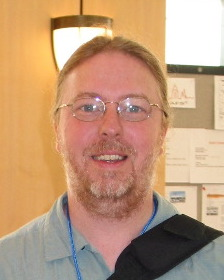
\includegraphics[width=\linewidth]{mugs/matt.jpg}
    \end{minipage}&
    \begin{minipage}{0.7\linewidth}
      Matt Newville, of course.  Without {\ifeffit} none of us would
      be having this much fun
    \end{minipage} \\
    \begin{minipage}{0.1\linewidth}
      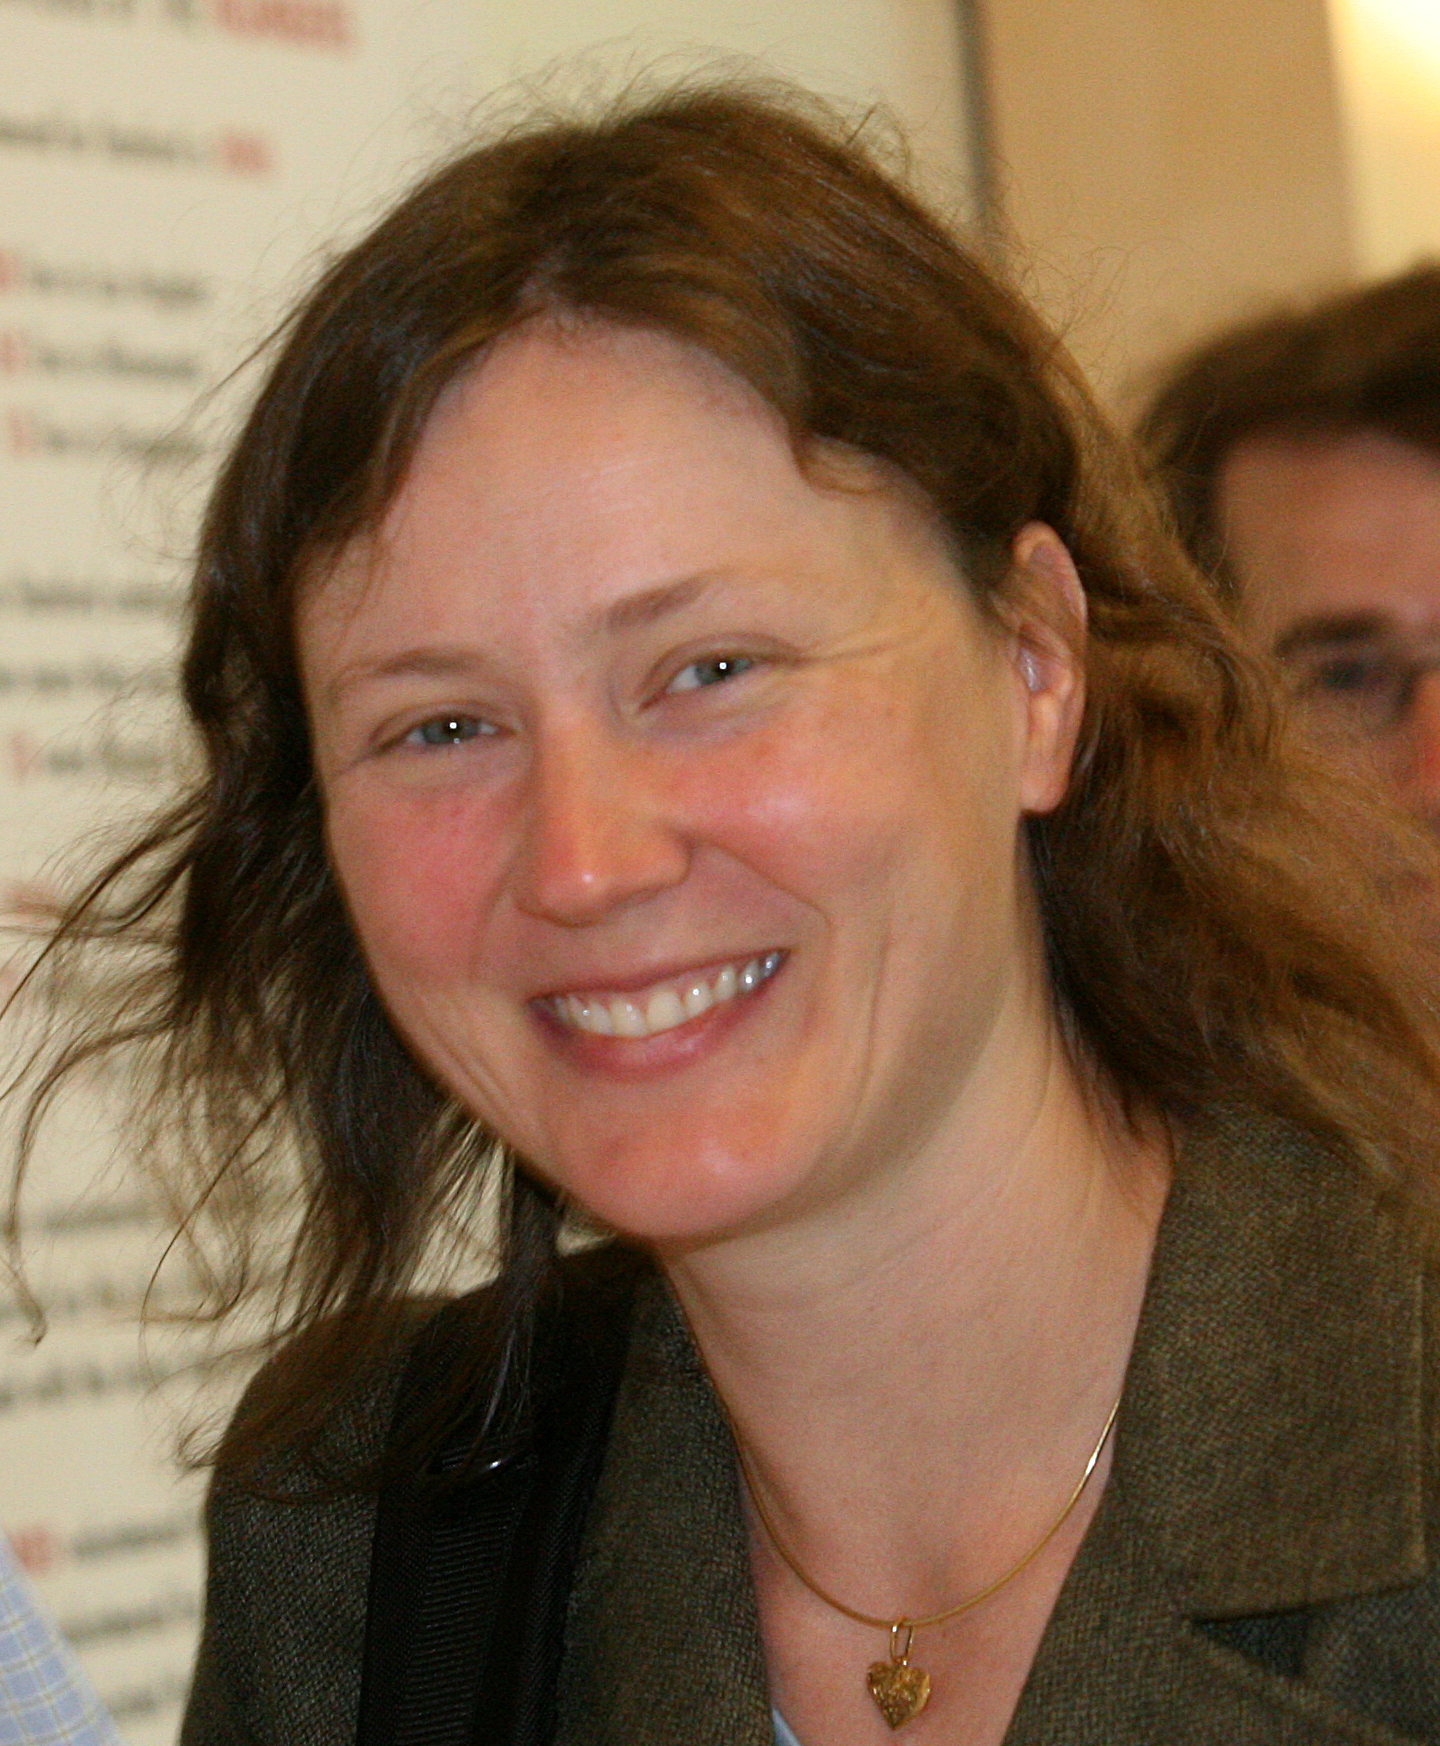
\includegraphics[width=\linewidth]{mugs/shelly.jpg}
    \end{minipage}&
    \begin{minipage}{0.7\linewidth}
      Shelly Kelly, bug finder extraordinaire and progenitor of several
      examples in this talk
    \end{minipage} \\
    \begin{minipage}{0.1\linewidth}
      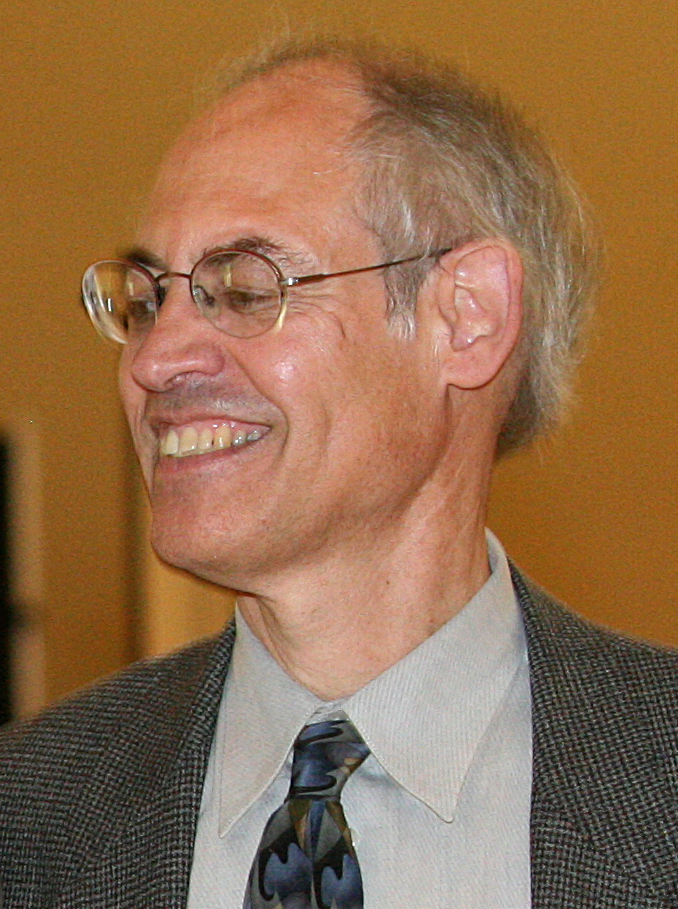
\includegraphics[width=\linewidth]{mugs/john.jpg}
    \end{minipage}&
    \begin{minipage}{0.7\linewidth}
      John Rehr and his group.  If we didn't have fun with {\feff}, we
      wouldn't have fun with {\ifeffit}
    \end{minipage} \\
    \begin{minipage}{0.1\linewidth}
      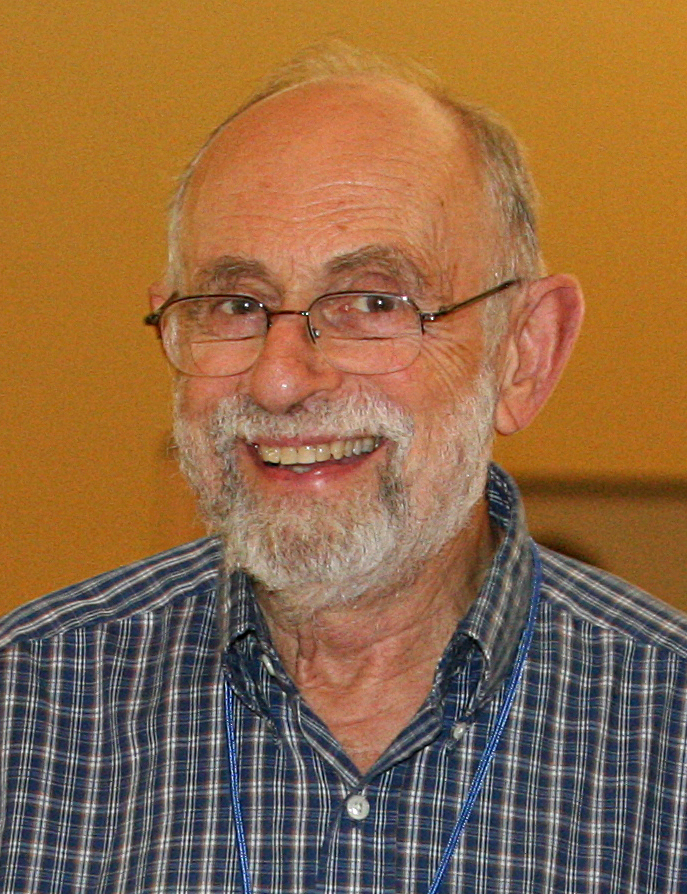
\includegraphics[width=\linewidth]{mugs/ed.jpg}
    \end{minipage}&
    \begin{minipage}{0.7\linewidth}
      Ed Stern, for teaching us all so well and for getting all this XAS
      stuff started in the first place
    \end{minipage}
  \end{tabular}

  \medskip

  \begin{itemize}
    \footnotesize
  \item The many users of my software: without years of feedback and
    encouragement, my codes would suck way more than they do
  \item The folks who make the great software I use to write my codes:
    \href{http://www.perl.org}{\color{Blue4}Perl},
    \href{http://wxperl.sourceforge.net/}{\color{Blue4}wxPerl},
    \href{http://www.gnu.org/software/emacs/}{\color{Blue4}Emacs},
    \href{http://ecb.sourceforge.net}{\color{Blue4}The Emacs Code Browser},
    \href{http://git-scm.com/}{\color{Blue4}Git},
    \href{http://github.com/}{\color{Blue4}GitHub}
  \item The folks who make the great software used to write this talk:
    \href{http://tug.ctan.org}{\color{Blue4}\LaTeX},
    \href{http://latex-beamer.sourceforge.net}{\color{Blue4}Beamer},
    \href{http://avogadro.sourceforge.net}{\color{Blue4}Avogadro},
    \href{http://www.gimp.org}{\color{Blue4}The Gimp},
    \href{http://www.gnuplot.info}{\color{Blue4}Gnuplot}
  \end{itemize}
\end{frame}

%\mode<handout>{\frame{\tableofcontents}}

%% \section*{Outline}
%% \begin{frame}
%%   \tableofcontents
%% \end{frame}


\section[Introduction]{Introduction}

%\subsection{Beamline}
\begin{frame}
  \frametitle{This Talk}
  
  \begin{block}{This is \textbf{NOT} the introductory talk}
    \begin{itemize}
    \item I assume you are a veteran of many XAS campaigns and that
      you already have your own data that you care about.
    \item I assume you are familiar with the EXAFS equation.
    \item I assume you understand XAS data processing and have done
      some EXAFS analysis.
    \item Some familiarity with {\ifeffit} or {\artemis} will help.
    \end{itemize}
  \end{block}

  \bigskip

  \begin{alertblock}{}
    \begin{center}
      The audience for this talk is interested in advanced techniques
      which will improve their use of their EXAFS data.
    \end{center}
  \end{alertblock}
\end{frame}

\begin{frame}
  \frametitle{This Talk}
  \begin{columns}
    \begin{column}{0.5\linewidth}
      %% fetch from http://waynocartoons.blogspot.com/2011_05_01_archive.html
      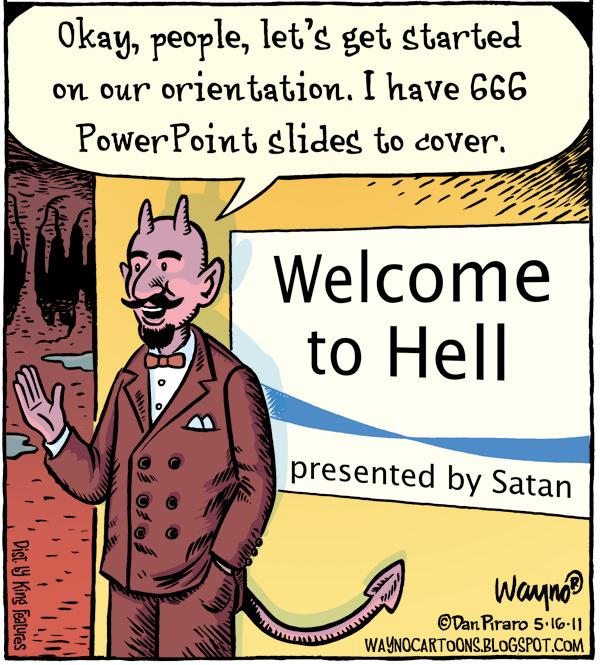
\includegraphics[width=\linewidth]{images/bz-panel-05-16-11-wno.jpg}
    \end{column}
    \begin{column}{0.5\linewidth}
      This is a long talk with some difficult content.  

      \bigskip

      We'll take a break in the middle.
    \end{column}
  \end{columns}
  \begin{bottomnote}[0.4][19.0]%
    Cartoon $\copyright$ Wayno and Dan Piraro
    \href{http://waynocartoons.blogspot.com/2011_05_01_archive.html}
    {\color{LightBlue4}{\ComputerMouse~}\texttt{http://waynocartoons.blogspot.com/2011\_05\_01\_archive.html}}
  \end{bottomnote}
\end{frame}

\begin{frame}[label=themultiples]
  \frametitle{The ``Multiples''}
  \begin{description}[Multiple]
  \item[Multiple $k$-weight] Co-refinement of the data using {\multiple}
    values of $k$-weighting in the Fourier Transform
  \item[Multiple Feff Calculations] Using {\multiple} runs of the
    {\feff} program to generate the theory used in your fitting
    model
  \item[Multiple Data Sets] Co-refinement of {\multiple} data sets --
    this may be data measured at multiple edges, multiple
    temperatures, etc.
  \item[Constraints Between Parameters] At the heart of an EXAFS
    fitting model are the relationships imposed between fitting
    parameters
  \item[Restraints on Parameters] Application of imperfect knowledge
    to influence the evaluation of a fit
  \end{description}
  \begin{block}{Using the ``multiples''}
    All of these are implemented in {\artemis} and will be
    discussed in this talk.
  \end{block}
\end{frame}



%\definecolor{MYcolor}{rgb}{0.8,0,0}
%\setbeamercolor{titlelike}{parent=pallette primary,fg=MYcolor}
\section[Statistics]{Statistical Considerations in EXAFS Analysis}

\subsection[Information]{Information}
\begin{frame}
  \frametitle{Information Content of EXAFS (I)} 

  \small
  Sometimes, we have {\color{Green4}\textit{beautiful}} data.  This is
  the merge of 5 scans on a 50\,nm film of GeSb on silica, at the Ge
  edge and measured in fluorescence at NSLS X23A2.\\~

  \begin{columns}
    \begin{column}{0.5\linewidth}
      \begin{center}
        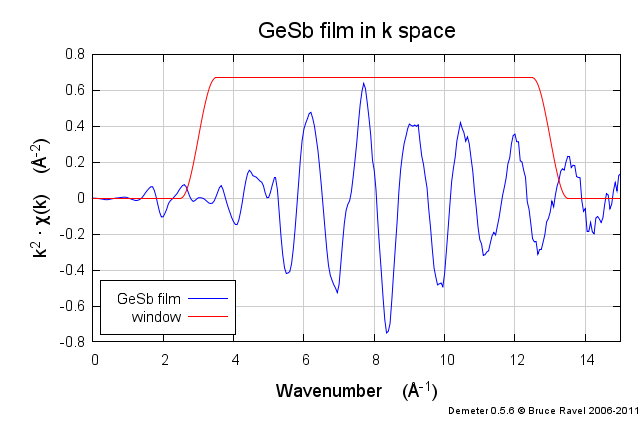
\includegraphics[width=0.8\linewidth]{info/gesb_chik.png}
      \end{center}
    \end{column}
    \begin{column}{0.5\linewidth}
      \begin{center}
        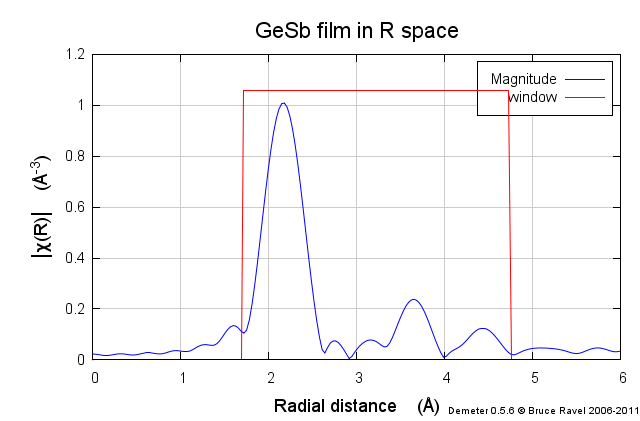
\includegraphics[width=0.8\linewidth]{info/gesb_chir.png}
      \end{center}
    \end{column}
  \end{columns}
  Here, I show a Fourier transform window of [3\,:\,13] and I suggest a
  fitting range of [1.7\,:\,4.7].  Applying the Nyquist criterion:
  \begin{equation}
    \notag N_{idp} \approx \frac{2\Delta k\Delta R}{\pi} \approx \alert{19}
  \end{equation}

  ~\\[-7ex]
  ~

  \begin{exampleblock}{}
    \begin{center}
      This gives us an upper bound of the information content of that
      portion of the EXAFS spectrum.
    \end{center}
  \end{exampleblock}
  \begin{bottomnote}[0.4][19.25]%
    These data are courtesy of Joseph Washington and Eric
    Joseph (IBM Research)
  \end{bottomnote}
\end{frame}

\begin{frame}
  \frametitle{Information Content of EXAFS (II)}
  \small
  Sometimes, we have less-than-beautiful data.  This is the merge of 42
  scans on a solution containing 3\,mM of Hg bound to a synthetic DNA
  complex, measured in fluorescence at APS 20BM.
  \begin{columns}
    \begin{column}{0.5\linewidth}
      \begin{center}
        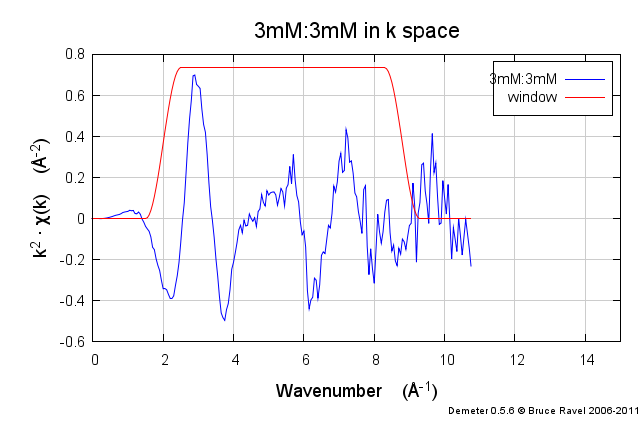
\includegraphics[width=0.8\linewidth]{info/hgdna_chik.png}
      \end{center}
    \end{column}
    \begin{column}{0.5\linewidth}
      \begin{center}
        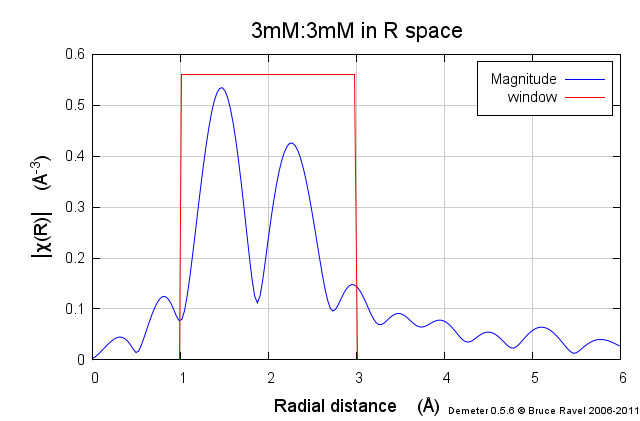
\includegraphics[width=0.8\linewidth]{info/hgdna_chir.png}
      \end{center}
    \end{column}
  \end{columns}
  Here, I show a Fourier transform window of [2\,:\,8.8] and I suggest a
  fitting range of [1\,:\,3].  Applying the Nyquist criterion:
  \begin{equation}
    \notag N_{idp} \approx \frac{2\Delta k\Delta R}{\pi} \approx \alert{8}
  \end{equation}

  ~\\[-7ex]
  ~

  \begin{exampleblock}{}
    \begin{center}
      This talk discusses strategies for dealing with severely limited
      information content.
    \end{center}
  \end{exampleblock}

  \begin{bottomnote}[0.7][19.0]%
    B.\ Ravel, et al., \textit{EXAFS studies of catalytic DNA sensors
      for mercury contamination of water}, Radiation Physics and
    Chemistry \textbf{78}:10 (2009) pp\ S75-S79.
    \doiref{10.1016/j.radphyschem.2009.05.024}[LightBlue4]
  \end{bottomnote}
\end{frame}

\begin{frame}
  \frametitle{What is This \textit{Nyquist Criterion} thingie?}

  Applying Fourier analysis to $\chi(k)$ means that we treat EXAFS as
  a signal processing problem.  If
  \begin{itemize}
  \item<1-> The signal is ideally packed \alert{\textbf{and}}
  \item<2-> The error in the fitting parameters is normally distributed
    \alert{\textbf{and}}
  \item<3-> We understand and can enumerate all sources of error
    \alert{\textbf{and}}
  \item<4-> We know the theoretical lineshape of our data
    \alert{\textbf{then}}
  \end{itemize}

  \medskip

  \onslide<5-6>{
    \begin{equation}
      \notag N_{idp} \approx \frac{2\Delta k\Delta R}{\pi}
    \end{equation}
  
    \medskip

    where, for EXAFS, $\Delta k$ is the range of Fourier transform and
    $\Delta R$ is the range in $R$ over which the fit is evaluated.
  }

  \begin{alertblock}<6>{Unfortunately ...}
    None of those conditions really get met in EXAFS.  $N_{idp}$ is,
    at best, an upper bond of the actual information content of the
    EXAFS signal.
  \end{alertblock}
  
\end{frame}

\subsection[Parameters]{Statistical Parameters}
\begin{frame}
  \frametitle{Statistical Parameters: Definitions}
  
  {\ifeffit} uses a Levenberg-Marquardt non-linear least-squares
  minimization, a standard $\chi^2$ fitting metric, and a simple
  definition of an R-factor:

  {\small
    \begin{align}
      \chi^2      =& \frac{N_{idp}}{\epsilon N_{data}}
                     \sum\limits_{i=min}^{max} 
                       \bigg[\Re\big(\chi_d(r_i)-\chi_t(r_i)\big)^2 + 
                             \Im\big(\chi_d(r_i)-\chi_t(r_i)\big)^2\bigg]
                     \label{eq:chisqr} \\
      \chi_\nu^2  =& \> \frac{\chi^2}{\nu} \label{eq:chinu} \\
      \nu         =& \> N_{idp} - N_{var} \label{eq:nu} \\
      \epsilon    =& \> \textrm{measurement uncertainty} \notag \\
      \mathcal{R} =& \frac{\sum\limits_{i=min}^{max} 
                             \bigg[\Re\big(\chi_d(r_i)-\chi_t(r_i)\big)^2 + 
                                   \Im\big(\chi_d(r_i)-\chi_t(r_i)\big)^2\bigg]}
                          {\sum\limits_{i=min}^{max} 
                             \bigg[\Re\big(\chi_d(r_i)\big)^2 + 
                                   \Im\big(\chi_d(r_i)\big)^2\bigg]} 
                     \label{eq:rfactor}
    \end{align}
  }
  \begin{block}{}
    In Gaussian statistics, assuming that $\epsilon$ has been measured
    correctly, a \textit{good fit} has $\chi_\nu^2\approx1$.
  \end{block}
\end{frame}

\begin{frame}
  \frametitle{An Obviously Good Fit}
  \begin{columns}[T]
    \begin{column}{0.4\linewidth}
      \begin{block}{}
        \begin{center}
          Here is a fit to the first two shells of copper metal at
          10\,K
        \end{center}
      \end{block}
      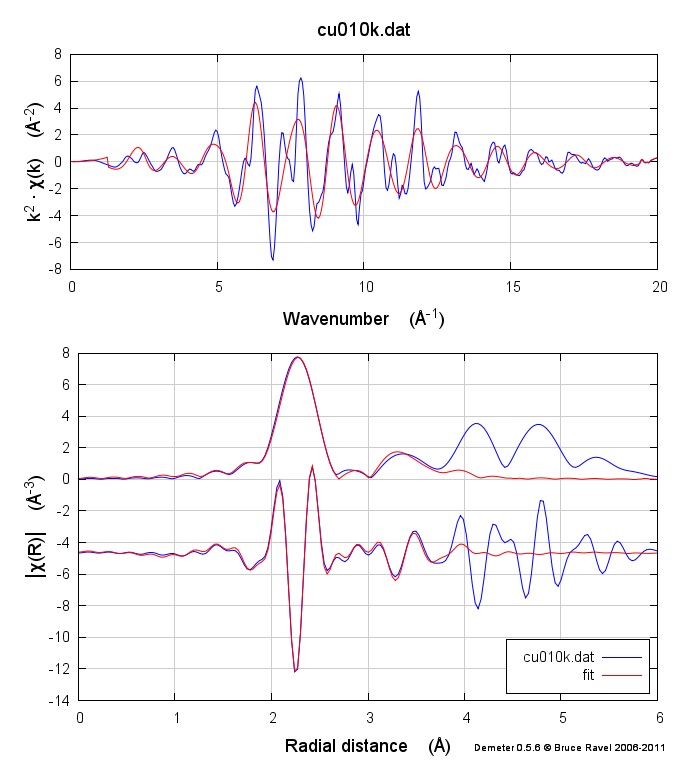
\includegraphics[width=\linewidth]{info/cufit.png}      
      %
      %\includegraphics[width=\linewidth]{info/cufit_chirre.png}      
    \end{column}
    \begin{column}{0.6\linewidth}
      \begin{center}
        This is an unambiguously good fit:
        
        \medskip

        \begin{tabular}{cc}
          $\mathcal{R}$ & 0.012 \\
          $N_{idp}$     & 16 \\
          $\nu$         & 12\\[1.5ex]
          $S_0^2$       & 0.87(6) \\
          $E_0$         & 6.04(62)\,eV \\
          $a$           & 3.6063(49)\,\AA \\
          $\Theta_D$    & 550(46)\,K \\
        \end{tabular}

        \medskip

        \onslide<2>{
          Yet \alert{$\chi_\nu^2 = 227.8$}\,!

          \bigskip
        
          \begin{alertblock}{What's goin' on here?}
            Why is $\chi_\nu^2$ for an obviously good fit so much larger
            than 1?
          \end{alertblock}
        }
      \end{center}
    \end{column}
  \end{columns}
\end{frame}

\begin{frame}
  \frametitle{Statistical Parameters: Fit Evaluation}

  \begin{columns}
    \begin{column}{0.3\linewidth}
      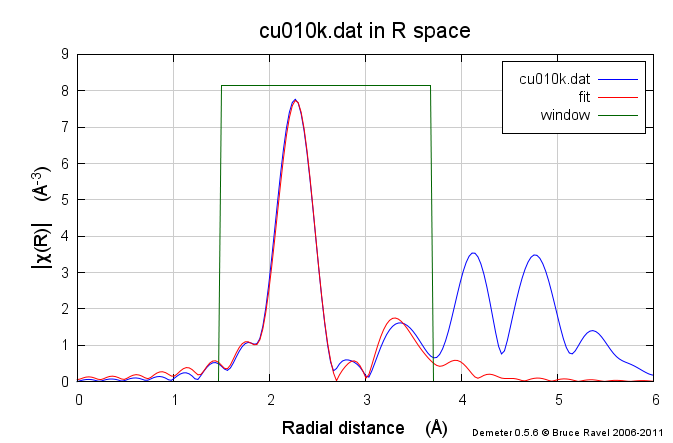
\includegraphics[width=\linewidth]{info/cufit_chirmag.png}      

      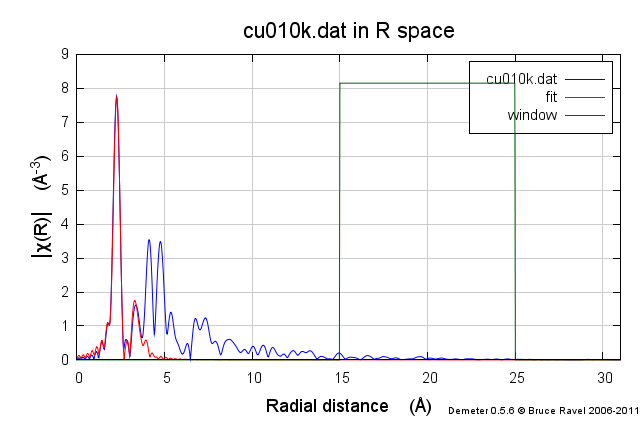
\includegraphics[width=\linewidth]{info/cu_chir0_31.png}      

      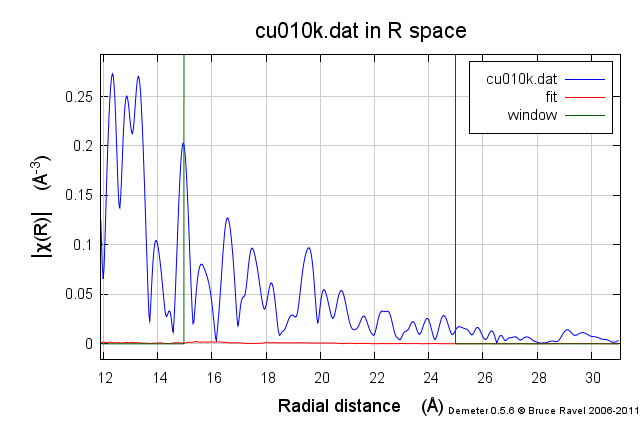
\includegraphics[width=\linewidth]{info/cu_chir12_31.png}      
    \end{column}
    \begin{column}{0.7\linewidth}
      The determination of measurement uncertainty is, perhaps, a bit
      hokey in {\ifeffit}.  It is the average of the signal between
      15\,\AA\ and 25\,\AA\ in the Fourier transform -- a range that
      probably does not include much signal above the noise.

      \bigskip

      Is that signal between 15\,\AA\ and 25\,\AA\ in copper metal?
      Perhaps....

      \bigskip

      In any case, this method ignores the following:
      \begin{itemize}
      \item Approximations and errors in theory
      \item Sample inhomogeneity
      \item Detector non-linearity
      \item Gremlins --- never forget about the gremlins! $\ddot\smile$
      \end{itemize}
    \end{column}
  \end{columns}
\end{frame}

\begin{frame}
  \frametitle{Statistical Parameters: Interpretation I}

  \begin{exampleblock}{}
    OK then ... what is the implication of $\epsilon$ never being
    evaluated correctly by {\ifeffit}?
  \end{exampleblock}

  \begin{enumerate}[<+->]
  \item $\chi^2_\nu$ is always somewhere between big and enormous.
  \item $\chi^2_\nu$ is impossible to interpret for a \textit{single} fit.
  \item $\chi^2_\nu$ {\color{Green4}\textbf{can}} be used to compare
    different fits.  A fit is improved if $\chi^2_\nu$ is
    significantly smaller.
  \item Error bars are taken from the diagonal of the covariance
    matrix.  If $\chi^2_\nu$ is way too big, the error bars will be way
    too small.  The error bars reported by {\ifeffit} have been scaled
    by $\sqrt{\chi^2_\nu}$.
  \item Thus the error bars reported by {\ifeffit} are of the
    {\color{Green4}``correct''} size if we assume that the fit
    is a {\color{Green4}``good fit''}.
  \end{enumerate}
\end{frame}

\begin{frame}
  \frametitle{Statistical Parameters: Interpretation II}

  \begin{exampleblock}{}
    \begin{center}
      How do we know if a fit is ``good''?
    \end{center}
  \end{exampleblock}
  \begin{itemize}[<+->]
  \item The current fit is an improvement over the previous fit if
    $\chi^2_\nu$ is sufficiently smaller.
  \item You should be suspicious of a fit for which $N_{var}$ is close
    to $N_{idp}$, i.e.\ a fit for which $\nu$ is small.
  \item All variable parameters should have values that are physically
    defensible and error bars that make sense.
  \item The results should be consistent with other things you know
    about the sample.
  \item The R-factor should be small and the fit should closely
    over-plot the data.  (That was redundant. $\ddot\smile$ )
  \end{itemize}
\end{frame}

\subsection[Other topics]{Other topics}
\begin{frame}
  \frametitle{Interpreting Error Bars}
  \begin{exampleblock}{}
    \begin{center}
      The interpretation of an error bar depends on the meaning of the
      parameter.
    \end{center}
  \end{exampleblock}

  \bigskip

  \begin{itemize}[<+->]
  \item A fitted $\sigma^2$ value of, say, $0.00567\pm0.00654$ is
    troubling.  That result means that $\sigma^2$ is ill-determined
    for that path and not even positive definite.  Yikes!
  \item On the other hand, a fitted $E_0$ value of, say,
    $0.12\pm0.34$ is just fine.  $E_0$ can be positive or negative.
    A fitted value consistent with 0 suggests you chose $E_0$ wisely
    back in {\athena}.
  \end{itemize}
  
\end{frame}

\begin{frame}
  \frametitle{Outside Knowledge}

  Because the information content of the XAS measurement is so
  limited, we are forced to incorporate knowledge from other
  measurements into our data analysis and its interpretation.

  \begin{itemize}
  \item Other XAS measurements --- for instance, the ``chemical
    transferability'' of $S_0^2$
  \item Diffraction tells us structure, coordination number, bond
    lengths, etc.
  \item Things like NMR, UV/Vis, and IR can tell us about the ligation
    environment of the absorber
  \item Common sense:
    \begin{itemize}
    \item $R_{NN}\ncong0.5$\,\AA, $R_{NN}\ncong4.0$\,\AA
    \item $\sigma^2 \nless 0$\,\AA$^2$
    \end{itemize}
  \item ... and anything else your (physical $\parallel$ chemical
    $\parallel$ biological $\parallel$ whatever) intuition tells you
  \end{itemize}
\end{frame}

% \begin{frame}
%   \frametitle{Other Analytical Approaches}
%   \begin{description}
%   \item[Bayesian approaches] Can be used to determine actual
%     information contents, can evaluate quality of variables chosen,
%     and so on...
%   \item[Wavelet transforms] Alternative to Fourier transforms.  Can be
%     used to emphasize certain aspects of the signal.  ``{\feff} wavelets''
%   \end{description}
% \end{frame}

\begin{frame}
  \frametitle{Artemis: Statistics in the log file}
  \small%
  \begin{center}
    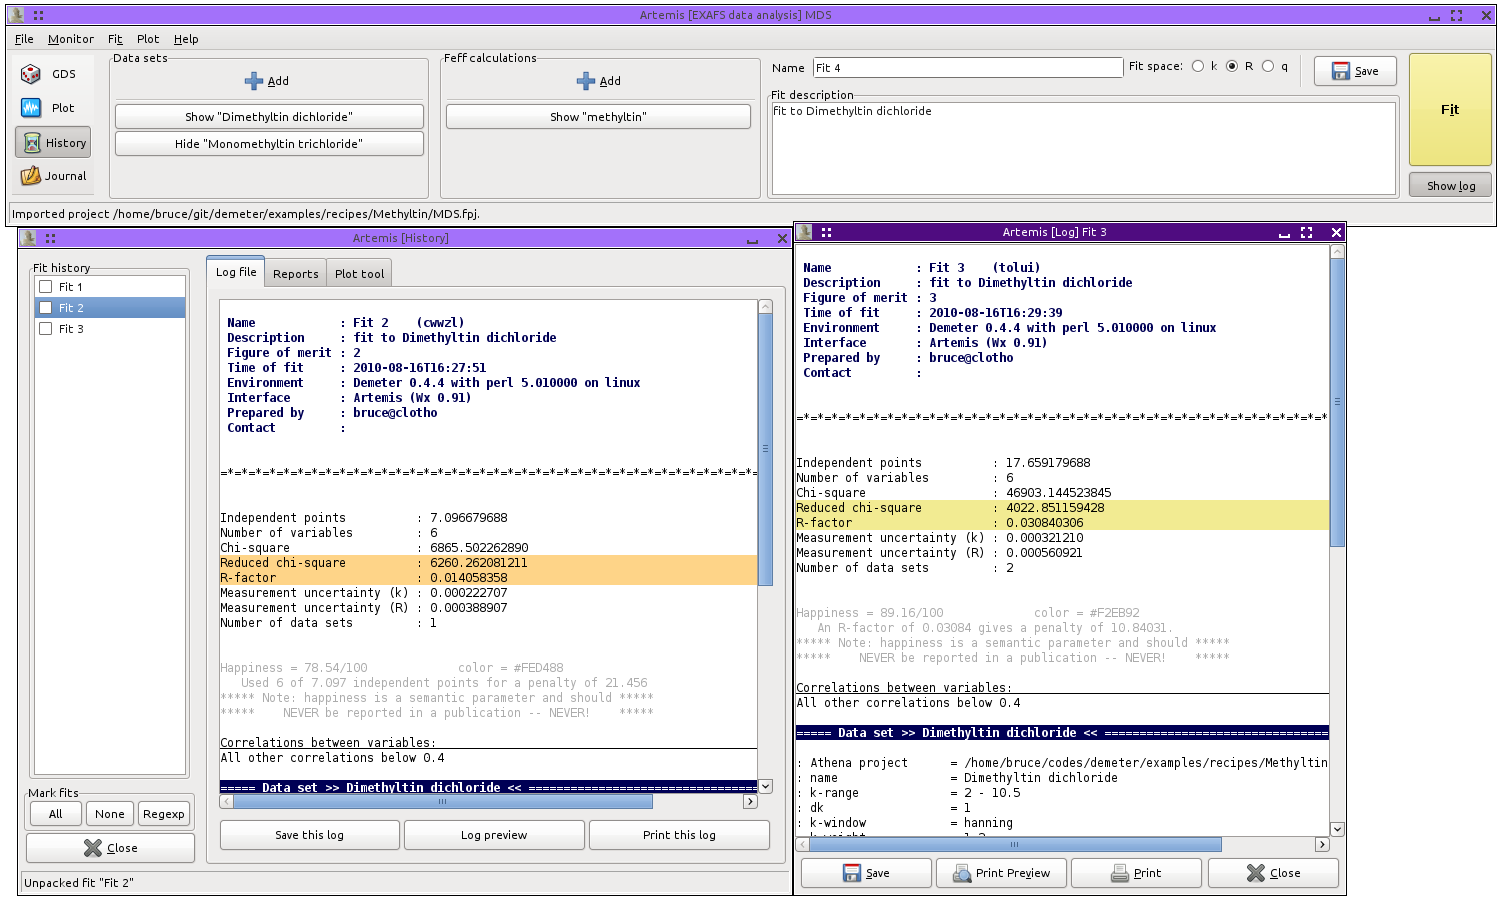
\includegraphics[width=0.9\linewidth]{info/log.png}

    Statistical information is reported in the log file.  The log from
    the most recent fit can be displayed by clicking the log button on
    the right side on the main window.  The log files from all fits in
    the project can be viewed by clicking the history button on the
    left side of the main window.
  \end{center}
\end{frame}


%\definecolor{MYcolor}{rgb}{0,0.5,0} %% dark green
\section[Ifeffit]{Evaluation of the EXAFS Equation in Ifeffit}
\begin{frame}
  \frametitle{The Path Expansion}

  {\ifeffit} is used to evaluate the EXAFS equation:
  {\small
    \begin{align}
      \chi(k,\Gamma) =& {\Im}\>\Biggl(\, %%\sum\limits_{\Gamma}
      { \frac{{\color{SlateBlue3}(N_\Gamma S_0^2)}{\color{Gold4}F_\Gamma(k)}}
        {2\,kR_\Gamma^2} }
      e^{i(2kR_\Gamma + {\color{Gold4}\Phi_\Gamma(k)})}
      e^{-2{\color{SlateBlue3}\sigma_\Gamma^2}k^2}
      e^{-2R_\Gamma/{\color{Gold4}\lambda(k)}}
      \Biggl) \\
      \chi_{\mathrm{theory}}(k) =& \sum\limits_{\Gamma}\chi(k,\Gamma) \notag\\
      R_\Gamma =& \> {\color{Gold4}R_{0,\Gamma}} +
      {\color{SlateBlue3}\Delta R_\Gamma} \\
      k =& N\sqrt{(E_0 - {\color{SlateBlue3}\Delta E_0})}
    \end{align}}

  \medskip

  $\chi_{\mathrm{theory}}(k)$ is the function that is fit to data by
  varying the fitting parameters using theory from {\feff} (the
  {\color{Gold4}terms in yellow-gray}).

  \bigskip

  \TheBigLesson
\end{frame}

\begin{frame}
  \frametitle{Flow control in Ifeffit}

  \begin{columns}
    \begin{column}{0.5\linewidth}
      Every trick in this talk exploits the fact that {\ifeffit}
      introduces this layer of abstraction between the
      {\color{SlateBlue3}path parameters} and the
      {\color{Green4}parameters of the fit}.

      \bigskip

      \begin{exampleblock}{}
        Virtually any clever idea you have for describing your data
        can be expressed using {\ifeffit}'s math expressions.
      \end{exampleblock}
    \end{column}
    \begin{column}{0.5\linewidth}
      \includegraphics[width=\linewidth]{images/ifeffit_control.pdf}      
    \end{column}
  \end{columns}
\end{frame}

%\definecolor{MYcolor}{rgb}{0,0.5,0} %% dark green
\section[MKW]{Multiple k-weight Fitting}
\subsection[Explain]{How Multiple k-weight Fitting Works}
\begin{frame}
  \frametitle{$k$-Dependence of Different Parameters}

  Let's look at the EXAFS equation again:

  {\small
    \begin{equation}
      \chi(k,\Gamma) = {\Im}\>\Bigl(\, %%\sum\limits_{\Gamma}
      { \frac{{\color{SlateBlue3}(N_\Gamma S_0^2)}{\color{Gold4}F_\Gamma(k)}}
        {2\,kR_\Gamma^2} }
      e^{i(2kR_\Gamma + {\color{Gold4}\Phi_\Gamma(k)})}
      e^{-2{\color{SlateBlue3}\sigma_\Gamma^2}k^2}
      e^{-2R_\Gamma/{\color{Gold4}\lambda(k)}}
      \Bigl) \notag
    \end{equation}}

  Different values of $k$-weight emphasize different regions of the
  spectrum. A $k$-weight of 3 puts more emphasis at high-$k$ in the
  evaluation of the fitting metric, while a $k$-weight of 1 tends to
  favor low-$k$.

  \begin{center}
    \begin{tabular}{cl}
      {\color{SlateBlue3}$S_0^2$}      &  same at all $k$ \\
      {\color{SlateBlue3}$\Delta R$}   & high $k$, goes as $k$ \\
      {\color{SlateBlue3}$\sigma^2$}   & high $k$, goes as $k^2$ \\
      {\color{SlateBlue3}$\Delta E_0$} & low $k$, goes as $\frac{1}{k}$ \\
    \end{tabular}
  \end{center}

  By using multiple $k$-weights, we hope to distribute the sensitivity
  of the evaluation of $\chi^2$ over the entire $k$ range and to make
  better use of the data available.
\end{frame}

\begin{frame}
  \frametitle{Evaluating A Multiple $k$-weight Fit}

  To evaluate an MKW fit, a $\chi^2$ is evaluated for each value of
  $k$-weighting used in the fit.
  
  {\small
    \begin{align}
      \chi^2_k =& \frac{N_{idp}}{\epsilon N_{data}}
      \sum\limits_{i=min}^{max} 
      \bigg[\Re\big(\chi_{d,k}(r_i)-\chi_{t,k}(r_i)\big)^2 + 
      \Im\big(\chi_{d,k}(r_i)-\chi_{t,k}(r_i)\big)^2\bigg]\Biggl|_{kw}
      \notag \\
      \chi^2_{total} =& \sum\limits_{\textrm{all kw}} \chi^2_k
    \end{align}}

  \begin{exampleblock}{}
    \begin{center}
      It's that simple!
    \end{center}
  \end{exampleblock}
\end{frame}

\subsection[Example]{A Multiple k-weight Example}
\begin{frame}[fragile,label=methyltin]
  \frametitle{Example: Methyltin in Solution}
  \begin{columns}[T]
    \begin{column}{0.6\linewidth}
      \qquad
      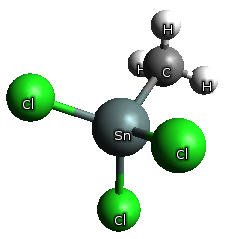
\includegraphics[width=0.3\linewidth]{mkw/monomethyltin.png}
      \qquad
      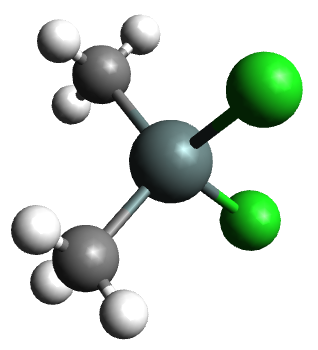
\includegraphics[width=0.3\linewidth]{mkw/dimethyltin.png}
      

      \begin{center}
        \begin{minipage}{0.6\linewidth}
          \begin{alltt}
\tiny
 {\color{Green4}TITLE     dimethyltin dichloride}
 {\color{SteelBlue4}HOLE}      1      1.0
 {\color{SteelBlue4}CONTROL}   1      1     1     1
 {\color{SteelBlue4}PRINT}     1      0     0     0
 {\color{SteelBlue4}RMAX}      6.0
 {\color{Purple3}POTENTIALS}
 {\color{Blue4}*    ipot   Z  element}
        0   50   Sn        
        1   17   Cl
        2    6   C
        3    1   H
 {\color{Purple3}ATOMS}
 {\color{Blue4}*   x       y       z}
   -0.027   2.146   0.014  2
    0.002  -0.004   0.002  0
    1.042  -0.716   1.744  2
   -2.212  -0.821   0.019  1
    1.107  -0.765  -1.940  1
    0.996   2.523   0.006  3
   -0.554   2.507  -0.869  3
   -0.537   2.497   0.911  3
    0.532  -0.365   2.641  3
    1.057  -1.806   1.738  3
    2.065  -0.339   1.736  3
          \end{alltt}
        \end{minipage}
      \end{center}
    \end{column}
    \begin{column}{0.4\linewidth}
      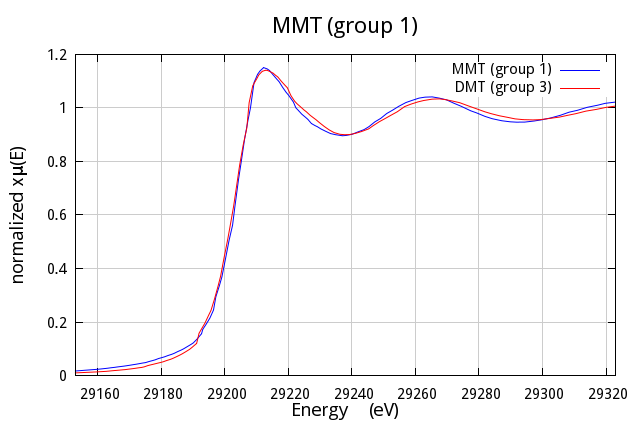
\includegraphics[width=0.85\linewidth]{mkw/data_xanes.png}      

      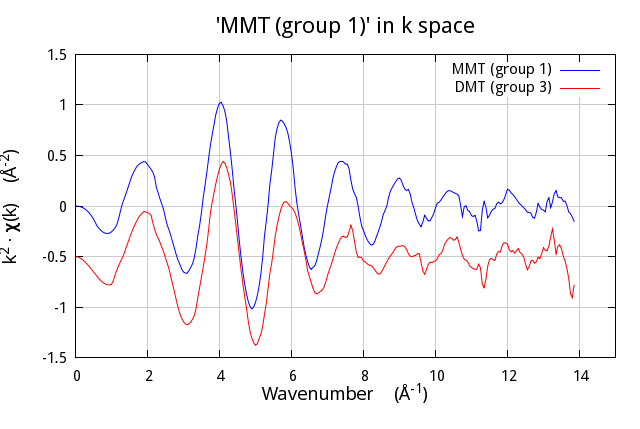
\includegraphics[width=0.85\linewidth]{mkw/data_chik.png}      

      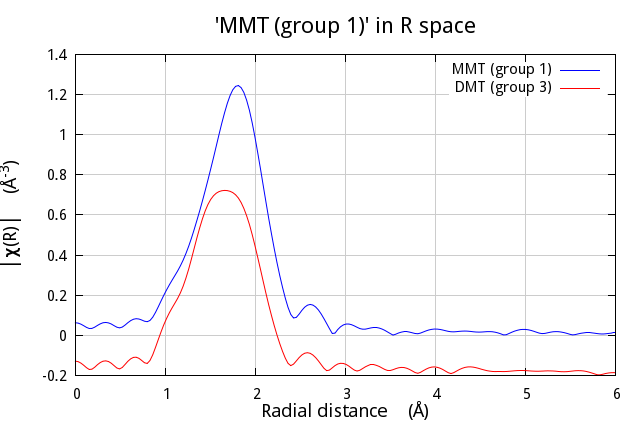
\includegraphics[width=0.85\linewidth]{mkw/data_chir.png}
    \end{column}
  \end{columns}

\end{frame}

\begin{frame}[fragile]
  \frametitle{Example: Dimethyltin Fit with kw=2}

  \begin{columns}[T]
    \begin{column}{0.6\linewidth}
      \small
      \quad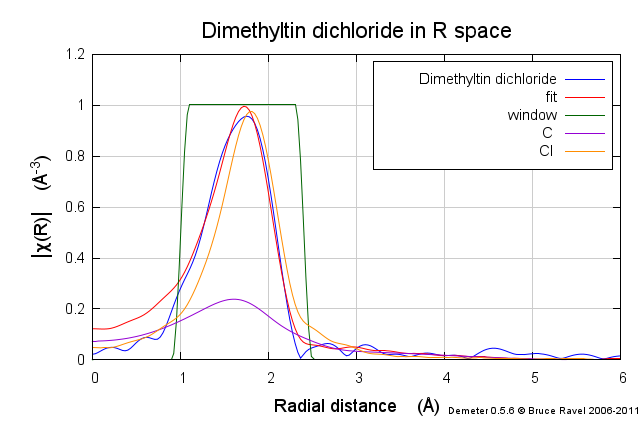
\includegraphics[width=0.7\linewidth]{mkw/fitkw2.png}

      The fit \textit{looks} OK, but it's actually kind of a mess.
      \begin{itemize}
        \small
      \item The $S_0^2$ value is way too big
      \item The $\sigma^2$ values are quite large
      \item One correlation is disturbingly high
      \end{itemize}
    \end{column}
    \begin{column}{0.4\linewidth}
      \tiny
\begin{alltt}
Fitting statistics
  \alert{Independent points          : 7.42676
  Number of variables         : 6}
  Chi-square                  : 2422.68
  Reduced Chi-square          : 1698.03
  R-factor                    : 0.01225
  Measurement uncertainty (k) : 0.00020
  Measurement uncertainty (R) : 0.00280

Guess parameters +/- uncertainties
  {\color{Blue3}amp     =  3.2595218 +/- 1.3818843}
  enot    =  3.9371728 +/- 3.7005334
  delr_c  =  0.1438966 +/- 0.1391769
  {\color{Blue3}ss_c    =  0.0544393 +/- 0.0378488}
  delr_cl = -0.0013874 +/- 0.0297003
  {\color{Blue3}ss_cl   =  0.0178517 +/- 0.0056183}

Correlations between variables:
         {\color{Blue3}amp and ss_cl   -->  0.9358}
        enot and delr_cl -->  0.8718
         amp and delr_c  -->  0.7556
      delr_c and ss_cl   -->  0.6849
         amp and ss_c    -->  0.6782
        enot and ss_c    --> -0.5909
       ss_cl and ss_c    -->  0.5551 
\end{alltt}
    \end{column}
  \end{columns}
  \begin{alertblock}{The problem?}
    Severe information limits!
  \end{alertblock}
\end{frame}

\begin{frame}[fragile]
  \frametitle{Example: Dimethyltin Fit with kw=1,2,3}

  \begin{columns}[T]
    \begin{column}{0.6\linewidth}
      \small
      \quad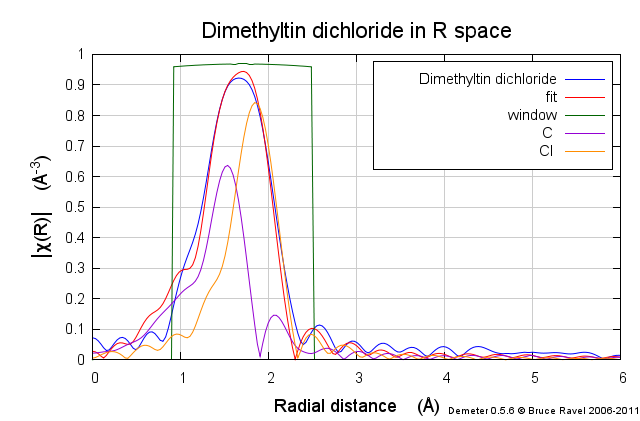
\includegraphics[width=0.7\linewidth]{mkw/fitkw123.png}

      This is much better.
      \begin{itemize}
      \item $S_0^2$ and $\sigma^2$ are more like what we anticipate
      \item The correlations are a bit more comforting
      \end{itemize}
    \end{column}
    \begin{column}{0.4\linewidth}
      \tiny
\begin{alltt}
Fitting statistics
  \alert{Independent points          : 7.42676
  Number of variables         : 6}
  Chi-square                  : 5213.30
  Reduced chi-square          : 3653.95
  R-factor                    : 0.01458
  Measurement uncertainty (k) : 0.00063
  Measurement uncertainty (R) : 0.00110

Guess parameters +/- uncertainties
  {\color{Green4}amp     =  1.2780228 +/- 0.2789866}
  enot    =  4.125484 +/- 2.5040201
  delr_c  = -0.0568480 +/- 0.0360530
  {\color{Green4}ss_c    =  0.00290554 +/- 0.0054193}
  delr_cl =  0.0202087 +/- 0.0241968
  {\color{Green4}ss_cl   =  0.0059542 +/- 0.0036629 }

Correlations between variables:
       ss_cl and ss_c   -->  0.8759
     delr_cl and enot   -->  0.8759
       ss_cl and amp    -->  0.8524
      delr_c and enot   -->  0.8329
        ss_c and amp    -->  0.8117
     delr_cl and delr_c -->  0.7922
\end{alltt}
    \end{column}
  \end{columns}
  \begin{exampleblock}{Problems remain}
    The information is still strained, but MKW certainly helps!
  \end{exampleblock}
\end{frame}

\begin{frame}
  \frametitle{Artemis: Multiple $k$-Weights}
  
  \begin{center}
    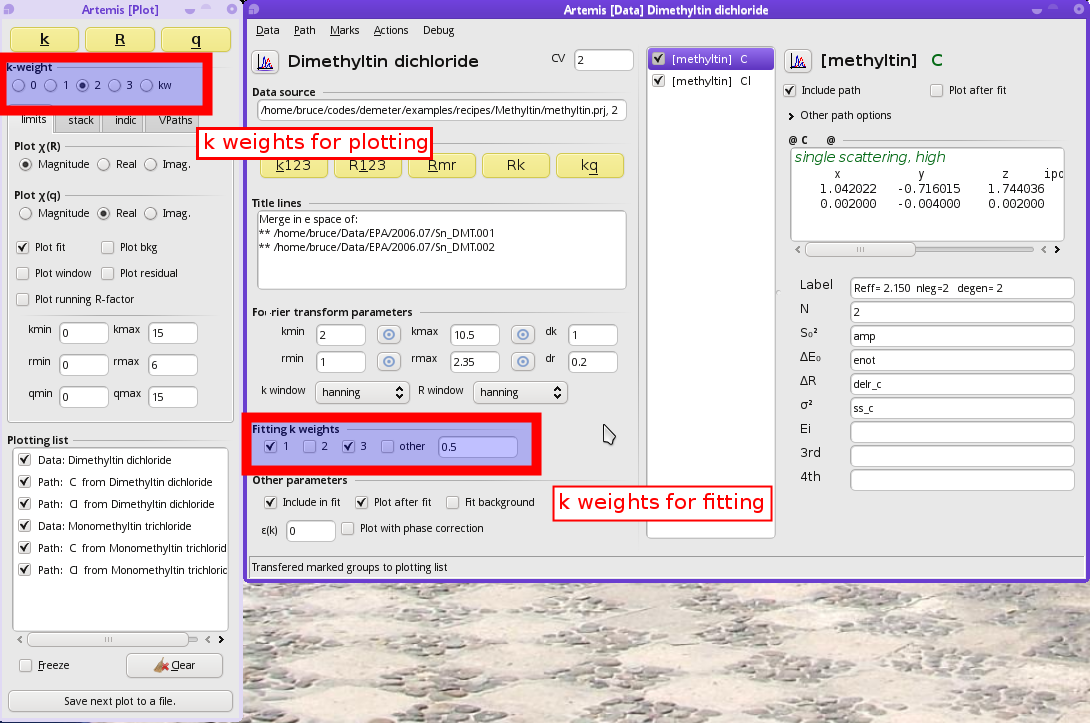
\includegraphics[width=0.9\linewidth]{artemis/mkw.png}

    Simply click any/all of the fitting $k$-weight buttons.\\
    Do not confuse them with the buttons that control k-weighting for
    plots.
  \end{center}
\end{frame}

%\definecolor{MYcolor}{RGB}{75,67,55}  %% dark brown
\section[MFC]{Multiple Feff Calculations}
\begin{frame}
  \frametitle{Absorbing Atoms in Multiple Environments}

  Consider situations like these:
  \begin{enumerate}
  \item A crystal with the absorbing atom in {\multiple} lattice
    positions
  \item A metalloprotein with {\multiple}, nonequivalent active sites
  \item An adsorbed metallic species that might be in {\multiple}
    ligation environments
  \item A physical mixture of {\multiple} species, e.g.\ dirt
  \item A thin film with {\multiple} layers
  \end{enumerate}

  \bigskip

  \begin{block}{A Feff input file has one-and-only-one absorbing
      site}
    A single {\feff} input file and a single {\feff} run cannot
    possibly be used to describe any of those situations.  How can we
    make progress?
  \end{block}
\end{frame}

\subsection[Explain]{How Multiple Feff Calculation Fitting Works}
\begin{frame}[fragile]
  \frametitle{\ybco: Multiple Lattice Positions}

  In {\ybco}, copper occupies 2 sites.  Site 1 is in a
  {\color{Blue3}four-fold planar} configuration.  Site 2 is near the
  center of a {\color{Blue3}square pyramid}.  The unit cell has
  \alert{one} Cu1 and \alert{two} Cu2 positions.
  
  \begin{center}

    \vskip -10pt

    \begin{minipage}{0.5\linewidth}
      \begin{block}{}
        \tiny
        \begin{alltt}
{\color{Green4}title YBCO: Y Ba2 Cu3 O7}
{\color{SteelBlue4}space} = P M M M
{\color{SteelBlue4}rmax}  = 7.2   {\color{SteelBlue4}a}=3.817 {\color{SteelBlue4}b}=3.882  {\color{SteelBlue4}c}=11.671
{\color{SteelBlue4}core}  = cu1
{\color{Purple4}atoms}
{\color{Blue4}! At.type   x        y       z       tag}
   Y       0.5      0.5     0.5
   Ba      0.5      0.5     0.1839
   Cu      0        0       0        cu1
   Cu      0        0       0.3546   cu2
   O       0        0.5     0        O1
   O       0        0       0.1589   O2
   O       0        0.5     0.3780   O3
   O       0.5      0       0.3783   O4
        \end{alltt}
      \end{block}
    \end{minipage}
  \end{center}

  This is handled naturally in {\ifeffit} after running {\feff} twice:

  \vskip -8pt
  
  \begin{columns}
    \begin{column}{0.5\linewidth}
      \scriptsize
      \begin{alltt}
  {\color{guessp}guess}  s0sqr = 0.9
  {\color{Purple4}path} \{
     {\color{Gold4}file}    site1/feff0001.dat
     {\color{Gold4}label}   1st path, site 1
     {\color{Gold4}s02}     s0sqr / 3
   \}
  {\color{Blue4}## all subsequent paths for site 1
  ## have} {\color{Gold4}s02}{\color{Blue4} * 1/3}
      \end{alltt}      
    \end{column}
    \begin{column}{0.5\linewidth}
      \scriptsize
      \begin{alltt}

  {\color{Purple4}path} \{
     {\color{Gold4}file}    site2/feff0001.dat
     {\color{Gold4}label}   1st path, site 2
     {\color{Gold4}s02}     2 * s0sqr / 3
   \}
  {\color{Blue4}## all subsequent paths for site 2
  ## have} {\color{Gold4}s02}{\color{Blue4} * 2/3}
      \end{alltt}      
    \end{column}
  \end{columns}
\end{frame}

\subsection[Example]{A Multiple Feff Calculation Example}
\begin{frame}
  \frametitle{Uranyl Ion Absorbed to Biomass}

  \begin{columns}[T]
    \begin{column}{0.5\linewidth}
      A uranyl solution brought into equilibrium with biomass will
      proportionate in a pH-dependent manner among hydroxyl,
      phosphoryl, and carboxyl ligands.
      \begin{itemize}
      \item Uranyl species tend to have 5 or 6 equatorial O's
      \item Phosphoryl ligands are monodentate
      \item Carboxyl ligands are bidentate
      \item Hydroxyls just dangle
      \end{itemize}
      \begin{alertblock}{}
        There is no way to find a \file{feff.inp} file for that!
      \end{alertblock}
    \end{column}
    \begin{column}{0.5\linewidth}
      \quad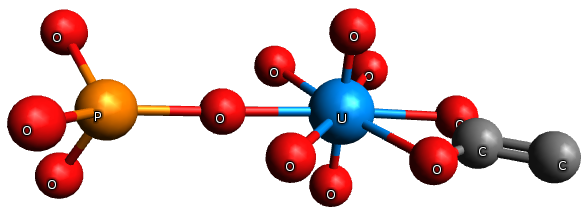
\includegraphics[width=0.8\linewidth]{mfc/uranyl.png}
      \begin{itemize}
      \item Use crystalline triuranyl diphoshate tetrahydrate for the
        phosphoryl component
      \item Use crystalline sodium uranyl triacetate for the carboxyl
        component 
      \item Use weights as fitting parameters to determine proportionation
      \end{itemize}
    \end{column}
  \end{columns}


  \begin{flushright}
    \begin{minipage}{0.5\linewidth}
      \tiny
      S.\ Kelly, et al. \textit{X-ray absorption fine-structure
        determination of pH dependent U-bacterial cell wall
        interactions}, Geochim.\ Cosmochim.\ Acta (2002)
      \textbf{66}:22, 3875--3891
    \end{minipage}
  \end{flushright}
\end{frame}

\begin{frame}
  \frametitle{Using Crystal Analogs as Feff Structures}
  \small
  \begin{columns}[T]
    \begin{column}{0.5\linewidth}
      Triuranyl diphoshate tetrahydrate contains a monodentate U-P moiety.
    \end{column}
    \begin{column}{0.5\linewidth}
      Sodium uranyl triacetate contains a bidentate U-C moiety.
    \end{column}
  \end{columns}

  \smallskip

  \begin{columns}[T]
    \begin{column}{0.5\linewidth}
      \begin{center}
        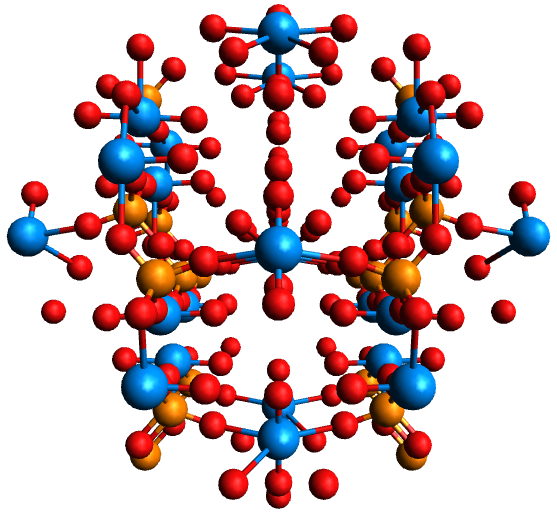
\includegraphics[width=0.4\linewidth]{mfc/upo4.png}

        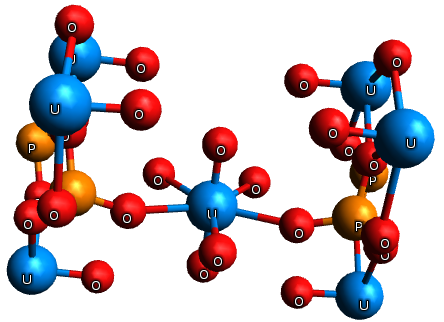
\includegraphics[width=0.5\linewidth]{mfc/upo4_full.png}
      \end{center}
    \end{column}
    \begin{column}{0.5\linewidth}
      \begin{center}
        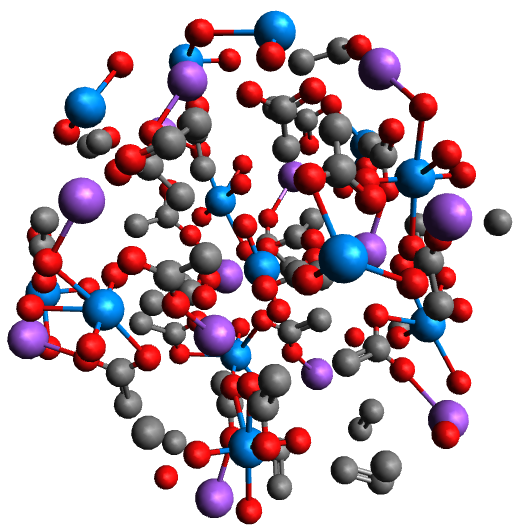
\includegraphics[width=0.4\linewidth]{mfc/NaU_triacetate_full.png}

        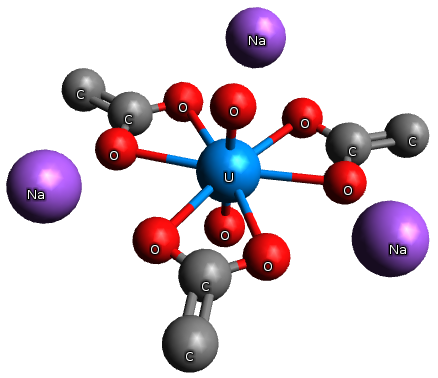
\includegraphics[width=0.5\linewidth]{mfc/NaU_triacetate.png}
      \end{center}
    \end{column}
  \end{columns}
  \begin{block}{The moral of this story ...}
    The structure used in the {\feff} calculation doesn't need to be
    ``perfect''.  Close is usually good enough to get started.
  \end{block}
\end{frame}

\begin{frame}
  \frametitle{Evaluating A Multiple Feff Calculation Fit}

  To evaluate an MFC fit, paths from each {\feff} calculation are used
  in the sum over paths used to compute the theoretical $\chi(k)$.
  
  {\small
    \begin{align}
      \chi_{th}(k) =& \sum\limits_\Gamma^{\textrm{(all structures)}} \>
      \sum\limits_\Gamma^{\textrm{(all included paths)}}\chi_\Gamma(k)
      \notag \\
      \chi^2      =& \frac{N_{idp}}{\epsilon N_{data}}
                     \sum\limits_{i=min}^{max} 
                       \bigg[\Re\big(\chi_d(r_i)-\chi_{th}(r_i)\big)^2 + 
                             \Im\big(\chi_d(r_i)-\chi_{th}(r_i)\big)^2\bigg]
                     \notag
    \end{align}}

  \begin{exampleblock}{}
    \begin{center}
      Again, it's that simple!
    \end{center}
  \end{exampleblock}
\end{frame}

\begin{frame}
  \frametitle{Artemis: Multiple Feff Calculations}

  \begin{center}
    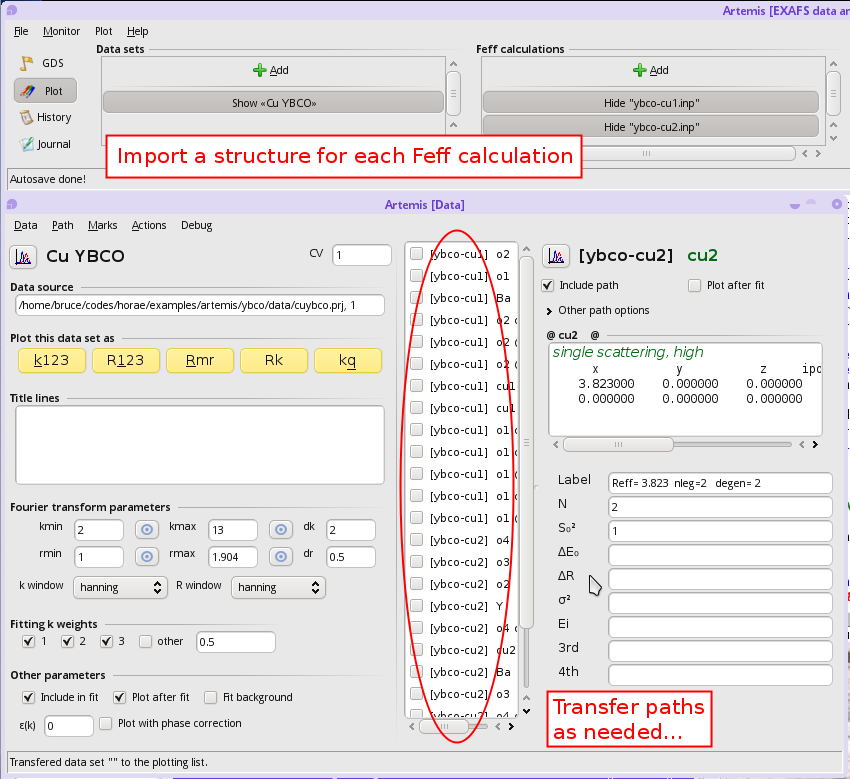
\includegraphics[width=0.6\linewidth]{artemis/mfc.png}

    Use as many {\feff} calculations as you need, run {\feff}, import
    and include whichever paths you need.  (\textit{Nota bene:} there
    is an out-of-the-box limit of 128 paths in {\ifeffit}.)
  \end{center}
\end{frame}

%\definecolor{MYcolor}{RGB}{204,135,33}  %%dirty orange
\section[MDS]{Multiple Data Sets}

\begin{frame}
  \frametitle{An Ensemble of Related Data Sets}

  Consider situations like these:
  \begin{enumerate}
  \item You have data at {\multiple} temperatures using a cryostat
    and/or a furnace
  \item You have data at {\multiple} pressures from a high pressure cell
  \item You have powders/films/solutions of {\multiple} stoichiometries
  \item You have data from an electrochemical sample at {\multiple} potentials
  \item You have data at {\multiple} edges of the same sample
  \end{enumerate}

  \bigskip

  \begin{block}{Some parameters may be related across data sets}
    Co-refining related data sets will dramatically increase the
    information content of the fit --- each data set \textbf{is} an
    independent measurement --- while not equivalently increasing the
    number of fitting parameters.
  \end{block}
\end{frame}

\subsection[Explain]{How Multiple Data Set Fitting Works}
\begin{frame}
  \frametitle{Example: Multiple Temperatures}

  I can co-refine the {\color{Green4}copper metal} data measured at
  many temperatures.  Here is the fit we saw earlier, extended to
  include 10\,K \textbf{and} 50\,K data:
  \begin{columns}
    \begin{column}{0.55\linewidth}
      \begin{itemize}
      \item $S_0^2$ and $E_o$ are the same for both data sets
      \item All $\sigma^2$ parameters for all paths at both
        temperatures are computed from \textit{one} variable Debye
        temperature.
      \item A linear dependence in temperature is assumed for the
        lattice expansion coefficient --- $\alpha(T) = m\cdot T+b$
      \end{itemize}
    \end{column}
    \begin{column}{0.45\linewidth}
      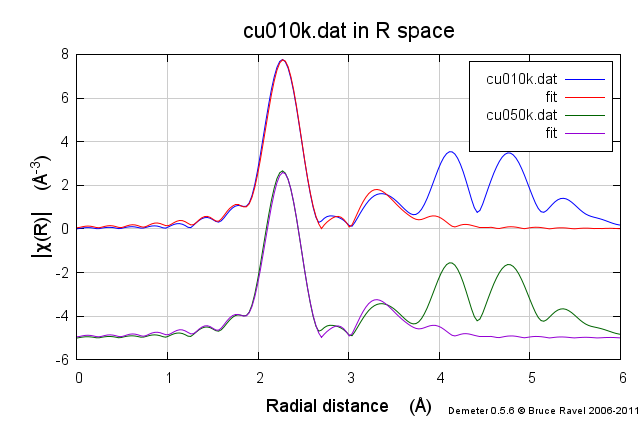
\includegraphics[width=\linewidth]{mds/cu10_150.png}
    \end{column}
  \end{columns}
  \begin{exampleblock}{}
    \begin{center}
      Twice as many independent points, only one more parameter!

      The more data, the better!
    \end{center}
  \end{exampleblock}
\end{frame}

\begin{frame}
  \frametitle{Evaluating A Multiple Data Set Fit}

  To evaluate an MDS fit, a $\chi^2$ is evaluated for each data set
  
  {\small
    \begin{align}
      \chi^2_D =& \frac{N_{idp}}{\epsilon N_{data}}
      \sum\limits_{i=min}^{max} 
      \bigg[\Re\big(\chi_{d,D}(r_i)-\chi_{t,D}(r_i)\big)^2 + 
      \Im\big(\chi_{d,D}(r_i)-\chi_{t,D}(r_i)\big)^2\bigg]\Biggl|_{\mathrm{data\ set}}
      \notag \\
      \chi^2_{total} =& \sum\limits_{\textrm{all data sets}} \chi^2_D
    \end{align}}

  \begin{exampleblock}{}
    \begin{center}
      Yet again, the evaluation of the fitting metric is a trivial
      extension of the simplest case.
    \end{center}
  \end{exampleblock}
\end{frame}


\subsection[Examples]{Further Multiple Data Set Examples}
%% re-show methyltin data, ball-n-sticks, feff.inp file
\againframe{methyltin}
\begin{frame}
  \frametitle{Example: Stoichiometry}

  I can co-refine {\color{Green4}forms of methyltin}, remembering that
  monomethyl tin has 1 Sn--C ligand and 3 Sn-Cl, while dimethyl tin
  has 2 and 2.
  \begin{columns}
    \begin{column}{0.55\linewidth}
      \begin{itemize}
      \item $S_0^2$ and $E_o$ are the same for both data sets
      \item I \textit{assert} that the $\sigma^2$'s for the Sn--C and
        Sn--Cl ligands are the same for di- and monomethyltin.
      \item Similarly, I \textit{assert} the bond lengths are the
        same.
      \end{itemize}
    \end{column}
    \begin{column}{0.45\linewidth}
      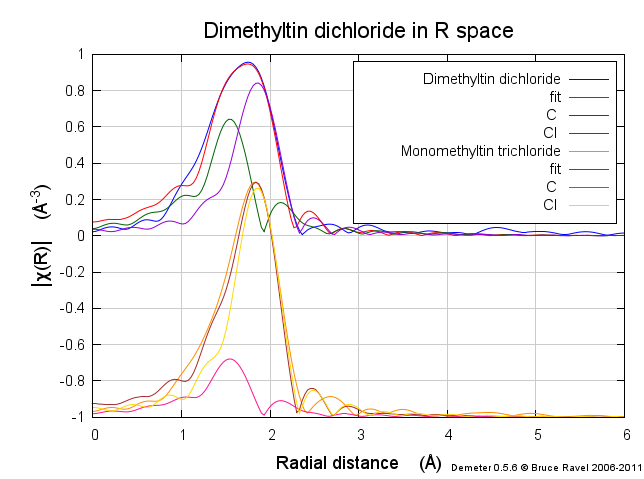
\includegraphics[width=\linewidth]{mds/methyltin.png}
    \end{column}
  \end{columns}
  \begin{exampleblock}{Twice the information, same number of parameters!}
    The simple assertion that the ligands are invariant between these
    samples adds considerable depth to the fitting model.  Is this
    assertion correct?  That is easily tested by lifting constraints
    on $\sigma^2$ and $\Delta R$ are comparing the fit results.
  \end{exampleblock}
\end{frame}

\begin{frame}
  \frametitle{Example: Two Edges}
  \begin{columns}[T]
    \begin{column}{0.35\linewidth}
      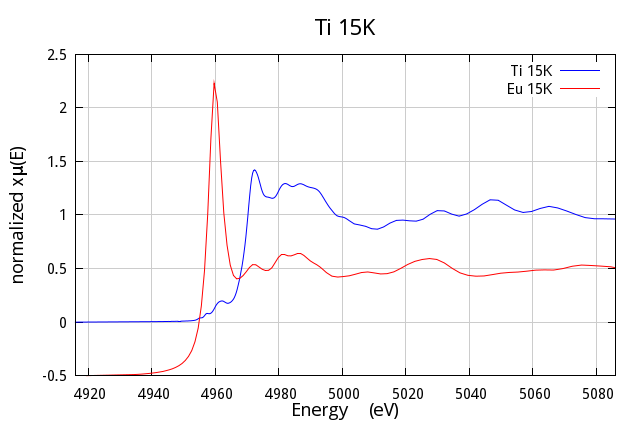
\includegraphics[width=\linewidth]{mds/eto_xanes.png}      

      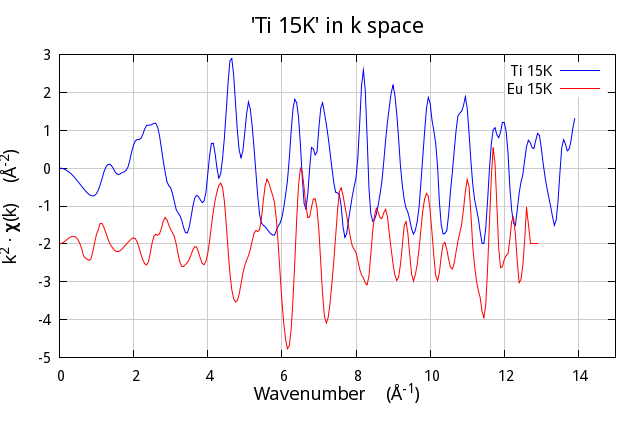
\includegraphics[width=\linewidth]{mds/eto_chik.png}      

      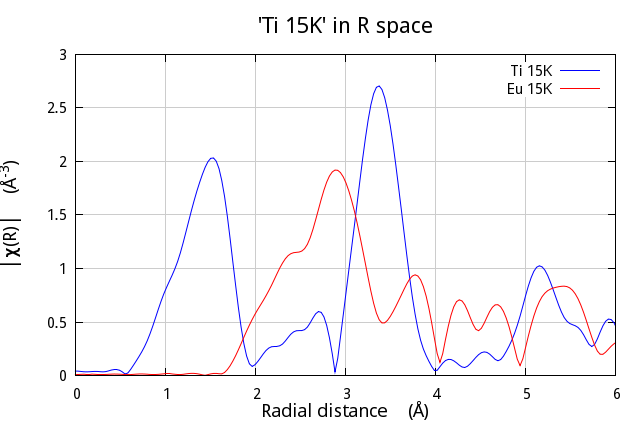
\includegraphics[width=\linewidth]{mds/eto_chir.png}
    \end{column}
    \begin{column}{0.65\linewidth}
      \small
      {\eto} is a regular cubic perovskite:

      \begin{center}
        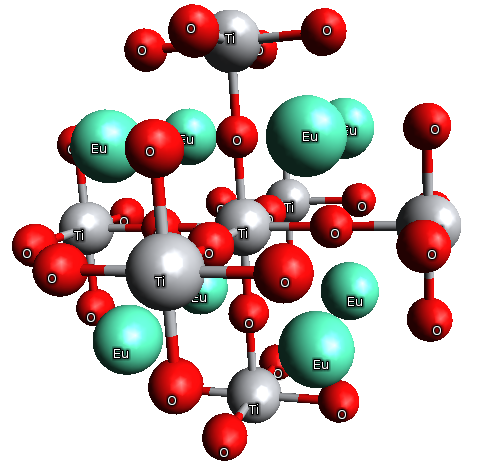
\includegraphics[width=0.4\linewidth]{mds/eto.png}
      \end{center}

      The data from the two edges share:
      \begin{itemize}
      \item A lattice constant
      \item An Eu--Ti $\sigma^2$
      \end{itemize}
      Other parameters must be independent for the two edges.

      \smallskip

      I have data from 15\,K to 500\,K, so I can combine {\multiple}
      temperatures, {\multiple} edges, \textbf{and} {\multiple}
      {\feff} calculations!
    \end{column}
  \end{columns}
\end{frame}

\begin{frame}
  \frametitle{Artemis: Multiple Data Sets (I)}

  If you have already imported data into {\artemis}, you can either
  change the data on which you are working or import additional data
  for a multiple data set fit,

  \begin{center}
    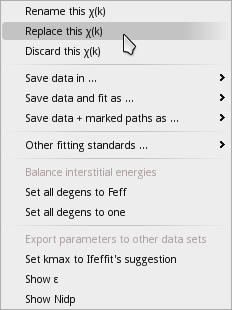
\includegraphics[width=0.2\linewidth]{artemis/change_data.png}\qquad
    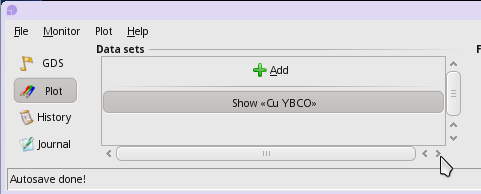
\includegraphics[width=0.4\linewidth]{artemis/data_import.png}
  \end{center}

  \begin{description}
  \item[Change] From the ``Data'' menu in the Data window, select the
    option to replace the $\chi(k)$.  This will open the file
    selection dialog.
  \item[New] Alternately, import data in the normal fashion.  It will
    be added to the list of Data sets and included in all subsequent
    fits.
  \end{description}
\end{frame}

\begin{frame}
  \frametitle{Artemis: Multiple Data Sets (II)}

  \begin{center}
    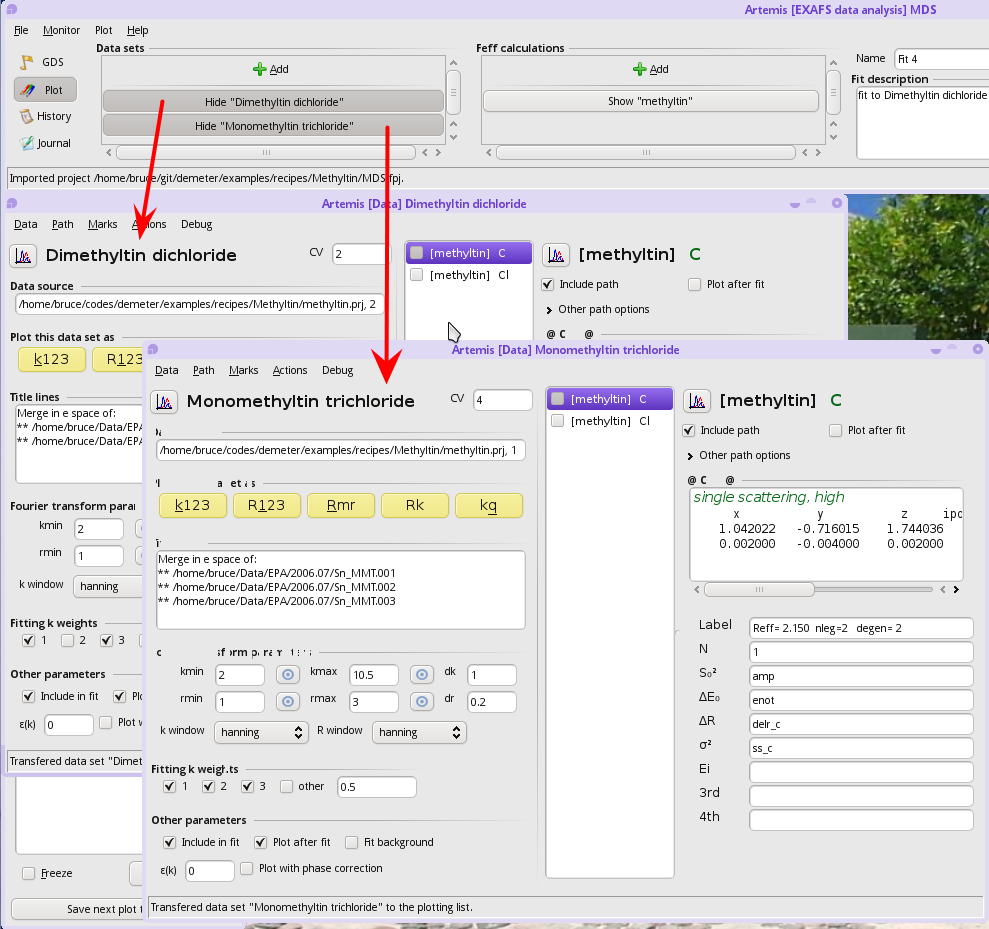
\includegraphics[width=0.6\linewidth]{artemis/mds.png}

    Use as many data sets calculations as you need.  Each data set
    needs one or more paths associated with it.  (\textit{Nota bene:}
    there is an out-of-the-box limit of 10 data sets in {\ifeffit}.)
  \end{center}
\end{frame}


%\definecolor{MYcolor}{RGB}{0,79,80}  %% dark teal
\section[Constraints]{Constraints Between Fitting Parameters}
\begin{frame}
  \frametitle{Building EXAFS Models}

  \begin{columns}
    \begin{column}{0.5\linewidth}
      \includegraphics[width=\linewidth]{images/ifeffit_control.pdf}      
    \end{column}
    \begin{column}{0.5\linewidth}
      All of {\ifeffit}'s magic happens in the {\color{SlateBlue3}blue
        steps}.  The effective use of MFC or MDS fitting, begins with
      clever model building.
    \end{column}
  \end{columns}
\end{frame}

\begin{frame}
  \frametitle{The Need for Constraints}

  Let's look at the EXAFS equation yet again:

  {\small
    \begin{equation}
      \chi(k,\Gamma) = {\Im}\>\Biggl(\, %%\sum\limits_{\Gamma}
      { \frac{{\color{SlateBlue3}(N_\Gamma S_0^2)}{\color{Gold4}F_\Gamma(k)}}
        {2\,kR_\Gamma^2} }
      e^{i(2kR_\Gamma + {\color{Gold4}\Phi_\Gamma(k)})}
      e^{-2{\color{SlateBlue3}\sigma_\Gamma^2}k^2}
      e^{-2R_\Gamma/{\color{Gold4}\lambda(k)}}
      \Biggl) \notag
    \end{equation}}

  \medskip

  For every path used in the fit, you must somehow evaluate 
  {\color{SlateBlue3}$N$},
  {\color{SlateBlue3}$S_0^2$},
  {\color{SlateBlue3}$\sigma^2$},
  {\color{SlateBlue3}$\Delta R$},
  {\color{SlateBlue3}$E_0$}.

  \medskip

  That's \alert{5 parameters per path}, but even for the beautiful
  GeSb data we had fewer than 20 independent points.

  \begin{block}{}
    \begin{center}
      Are we doomed?
    \end{center}
  \end{block}
  
  \onslide<2>{
    No.

    \bigskip

    \TheBigLesson
  }
\end{frame}

\begin{frame}
  \frametitle{The Simplest Constraints}

  Although each of 
  {\color{SlateBlue3}$N$},
  {\color{SlateBlue3}$S_0^2$},
  {\color{SlateBlue3}$\sigma^2$},
  {\color{SlateBlue3}$\Delta R$},
  {\color{SlateBlue3}$E_0$}.
  must be evaluated for each path, they are not necessarily
  independent parameters for each path.

  \bigskip

  Consider the copper metal we have already seen in this talk:
  \begin{description}
  \item[$S_0^2$] This is a parameter of the central atom and has
    something to do with the relaxation of electrons around the
    core-hole.  In copper metal, {\color{SlateBlue3}$S_0^2$} is
    the same for all paths.
  \item[$E_0$] In a single data set, single {\feff} calculation fit,
    this parameter is used to align the wavenumber grids of the data
    and theory.  In copper metal, {\color{SlateBlue3}$E_0$} is the
    same for all paths.
  \end{description}
  \begin{exampleblock}{}
    {\color{SlateBlue3}$S_0^2$} and {\color{SlateBlue3}$E_0$}
    represent the simplest kind of constraint --- parameters that are
    the same for each path.
  \end{exampleblock}

\end{frame}

\begin{frame}
  \frametitle{Slightly More Interesting Constraints}

  Copper metal also demonstrates simple constraints between paths
  involving math expressions:
  \begin{columns}
    \begin{column}{0.4\linewidth}
      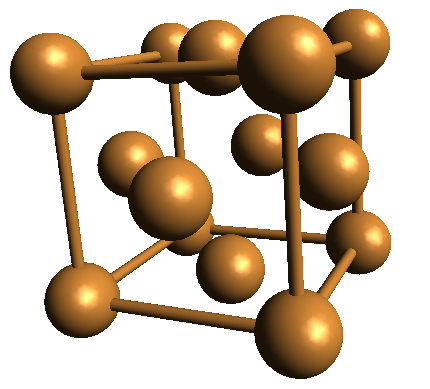
\includegraphics[width=\linewidth]{constraints/cu.png}      
    \end{column}
    \begin{column}{0.6\linewidth}
      \begin{description}[xyz]
      \item[$\Delta R$] As a highly symmetric, cubic metal, a volume
        expansion coefficient can be used to describe all path
        lengths. {\color{Green4}$\Delta R = \alpha*R_{eff}$}
      \item[$\sigma^2$] As a monoatomic metal, the mean square
        deviations in each path length can be described by the Debye
        temperature. {\color{Green4}$\sigma^2 = \debye(T, \Theta_D)$}
      \end{description}
    \end{column}
  \end{columns}
  
  \begin{block}{Path geometry}
    {\ifeffit} is clever enough to use the correct values for
    $R_{eff}$ (the path length used in the {\feff} calculation) and
    the reduced mass as path parameter math expressions are evaluated
    for each path.
  \end{block}
\end{frame}

\begin{frame}
  \frametitle{Model Building For Fun and Profit (I)}

  The uranyl problem requires multiple {\feff} calculations.  Making
  effective use of those calculations requires interesting
  constraints.

  \begin{center}
    \quad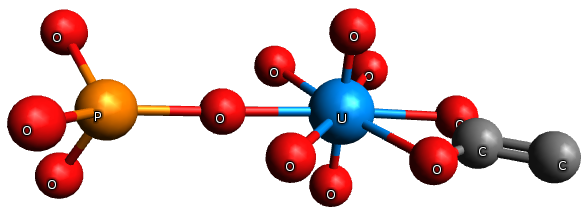
\includegraphics[width=0.7\linewidth]{mfc/uranyl.png}
  \end{center}

  \begin{itemize}
  \item The equatorial oxygen associated with a phosphoryl ligand
    is shorter than for a carboxyl ligand
  \item The posphoryl ligand is monodentate, thus $N_P = N_{short}$
  \item The carboxyl is bidentate, thus $N_c = N_{long}/2$
  \item If we assert that there are 6 equatorial oxygen atoms,
    then $N_{short} + N_{long} = 6$
  \end{itemize}
\end{frame}

\begin{frame}[fragile]
  \frametitle{Model Building For Fun and Profit (II)}

  \begin{center}
    \quad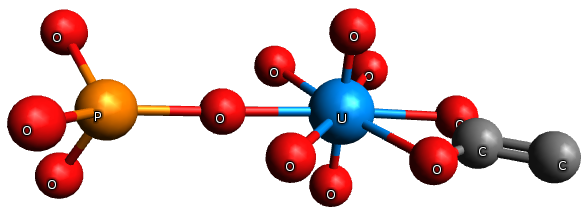
\includegraphics[width=0.7\linewidth]{mfc/uranyl.png}
  \end{center}

  \begin{block}{}
    \begin{alltt}
    \scriptsize
     {\color{setp}set}      n\_eq     = 6
     {\color{guessp}guess}    n\_short  = 3
     {\color{defp}def}      n\_long   = n\_eq - n\_short
     {\color{defp}def}      n\_p      = n\_short
     {\color{defp}def}      n\_c      = n\_long / 2

     {\color{guessp}guess}    ss\_short = 0.003
     {\color{defp}def}      ss\_long  = ss\_short
    \end{alltt}
  \end{block}

  We have described the coordination numbers and $\sigma^2$ for the
  equatorial oxygen atoms with a minimal number of
  {\color{guessp}guess}es.  The constraints on $\sigma^2$ and
  $N_{eq}$ can be lifted easily by switching a {\color{setp}set} or
  a {\color{defp}def} to a {\color{guessp}guess}.
\end{frame}
  
\begin{frame}
  \frametitle{Artemis: Specifying Constraints}

  \begin{center}
    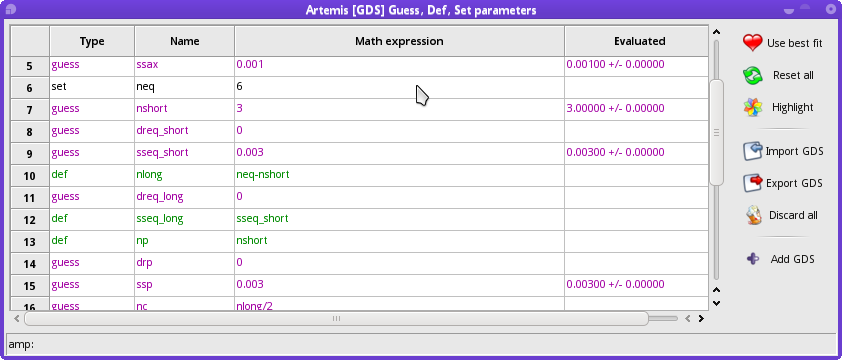
\includegraphics[width=\linewidth]{artemis/constraint.png}

    Constraints are implemented as {\color{defp}def} parameter math
    expressions.  (Path parameters can also be expressed as math
    expressions.)  {\ifeffit}'s math expressions are quite expressive.
  \end{center}
\end{frame}


%\definecolor{MYcolor}{RGB}{49,49,96}   %% dark purple
\section[Restraints]{Restraints On Fitting Parameters}
\begin{frame}
  \frametitle{Using Imperfect Knowledge}

  {\ifeffit} allows the incorporation of imprecise
  \alert{prior knowledge} by adding restraints in quadrature
  to the fitting metric.

  {\small
    \begin{align}
      \chi^2_{data} =& \frac{N_{idp}}{\epsilon N_{data}}
                      \sum\limits_{i=min}^{max} 
                        \bigg[\Re\big(\chi_d(r_i)-\chi_t(r_i)\big)^2 + 
                              \Im\big(\chi_d(r_i)-\chi_t(r_i)\big)^2\bigg]
                      \notag \\
     \chi^2 =& \> \chi^2_{data} + \sum\limits_{j}\Big[\frac{\lambda_{0,j} -
       \lambda_j}{\delta\lambda_j}\Big]^2 \label{eq:restraint}
   \end{align}
  }
  \begin{center}
    \begin{tabular}{cl}
      $\lambda_0$     & prior knowledge \\
      $\lambda$       & fitted value    \\
      $\delta\lambda$ & confidence      \\
    \end{tabular}
  \end{center}
  \begin{block}{The meaning of $\delta\lambda$}
      As $\delta\lambda\rightarrow\infty$, a restraint becomes unimportant.

      As $\delta\lambda\rightarrow0$, you admit no prior knowledge.
  \end{block}
\end{frame}

\begin{frame}[fragile]
  \frametitle{Restraints: A simple example}

  Suppose you have reason to believe that $0.6 < S_0^2 < 1.0$.

  \medskip

  \begin{description}[aaa]
  \item[Enforce this with ``hard-wall'' boundaries]~\\
    \begin{block}{}
\begin{alltt}
    \scriptsize
     {\color{guessp}guess} S0sqr = 0.8
     {\color{SteelBlue4}path}(1, S02 = {\color{Gold4}max}(0.6, {\color{Gold4}min}(1.0, S0sqr) ) )
\end{alltt}
    
      \footnotesize
      If the fitted value of $S_0^2$ strays out of bounds, error bars
      cannot be properly calculated.
    \end{block}
  \item[Apply a restraint, added in quadrature with $\chi^2_{data}$]~\\
    \begin{block}{}
\begin{alltt}
    \scriptsize
     {\color{guessp}guess}    S0sqr = 0.8
     {\color{setp}set}      scale = 2000
     {\color{restrainp}restrain} S0sqr\_res = scale * {\color{Gold4}penalty}(S0sqr, 0.6, 1.0)
     {\color{SteelBlue4}path}(1, S02 = S0sqr)
\end{alltt}
    \end{block}
    \begin{columns}
      \begin{column}{0.5\linewidth}
        \quad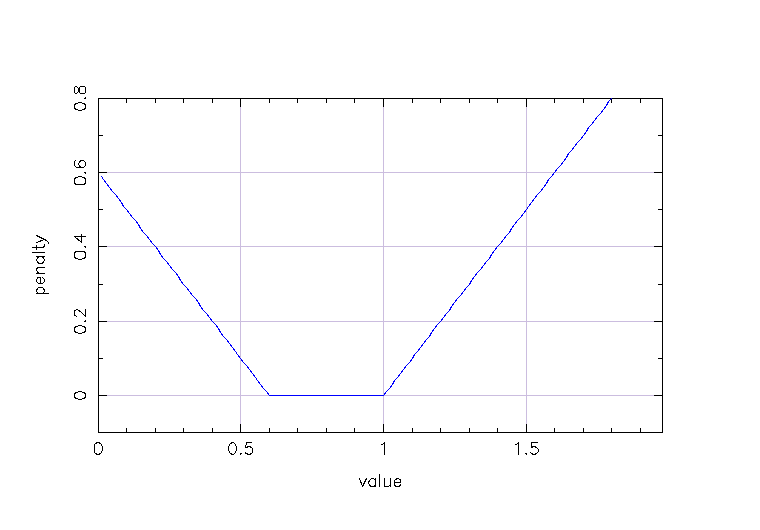
\includegraphics[width=0.8\linewidth]{restraints/penalty.png}
      \end{column}
      \begin{column}{0.4\linewidth}
        \small
        $S_0^2$ is encouraged to stay in bounds to avoid a penalty to
        $\chi^2$, but error bars can be properly evaluated when $S_0^2$
        strays.
      \end{column}
    \end{columns}
  \end{description}

\end{frame}

\begin{frame}[fragile]
  \frametitle{Restraints: A simple example (continued)}

  \small
  The assumption of ``chemical transferability'' of $S_0^2$ may be
  suspect, particularly if the known standard used to determine
  $S_0^2$ is prepared differently from the unknown.

  \bigskip

  Restrain $S_0^2$ to be like the standard
  \begin{block}{}
    \begin{alltt}
    \scriptsize
     {\color{guessp}guess}    S0sqr = 0.9
     {\color{setp}set}      S0sqr\_known = 0.876
     {\color{setp}set}      scale = 2000
     {\color{restrainp}restrain} S0sqr\_res = scale * (S0sqr - SOsqr\_known)
    \end{alltt}
  \end{block}

  \medskip

  Again, \texttt{S0sqr\_res} is added in quadrature with $\chi^2$.

  \medskip

  \onslide<2>{
    \begin{alertblock}{}
      \begin{center}
        How big should the \texttt{scale} be?
      \end{center}
    \end{alertblock}

    \medskip

    I don't have a good answer.  The square root of $\chi^2$ evaluated
    without the restraint seems to be a good size.  In the end, it
    depends upon how much trust you place on the restraint.
  }
\end{frame}

\begin{frame}[fragile]
  \frametitle{Restraints: Bond Valence Sums}

  The Bond Valence relates the valence of an ion to its ligand bond
  lengths using empirical parameters as determined by Brown and
  Altermatt, Acta Cryst.\ B41 (1985) pp.~244--247:

  \begin{equation}
    \label{eq:bvs}
    V_i = \sum\limits_{j=1}^N \exp\Big(\frac{R'_{ij} - R_{ij}}{0.37}\Big)
  \end{equation}

  0.37 and $R'_{ij}$ are empirical parameters, $R'_{ij}$ is
  different for each kind of pair, i.e.\ Fe--S, Ni--O, etc.
  Tetrahedral coordination involves different distances and valence
  than octahedral.

  \bigskip

  Octahedral iron example
  \begin{block}{}
    \begin{alltt}
    \scriptsize
     {\color{setp}set}      valence = 2
     {\color{setp}set}      rij     = 1.734  {\color{Blue4}# R'ij for Fe(2+)-O}
     {\color{setp}set}      rnot    = 2.14
     {\color{setp}set}      scale   = 1000
     {\color{guessp}guess}    delr    = 0.0
     {\color{restrainp}restrain} bvs     = valence - 6 * exp( (rij - (rnot+delr)) / 0.37 )
    \end{alltt}
  \end{block}

\end{frame}

\begin{frame}[fragile]
  \frametitle{Model Building For Fun and Profit (III)}

  From a literature survey, we know that the short and long equatorial
  oxygen bonds tend to be about 2.32\,\AA\ and 2.45\,\AA\ in uranyl
  complexes.

  \medskip

  \begin{center}
    \quad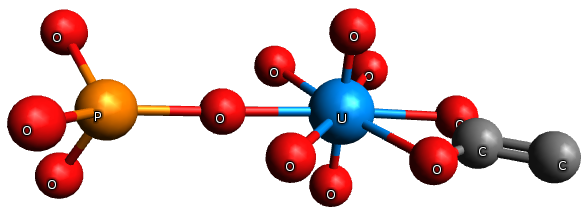
\includegraphics[width=0.7\linewidth]{mfc/uranyl.png}
  \end{center}

  Uranyl coordination parameters
  \begin{block}{}
    \begin{alltt}
    \scriptsize
     {\color{guessp}guess}      r\_short     = 2.32
     {\color{guessp}guess}      r\_long      = 2.45
     {\color{restrainp}restrain}   r\_short\_res = scale * penalty(r\_short, 2.30, 2.34)
     {\color{restrainp}restrain}   r\_long\_res  = scale * penalty(r\_short, 2.43, 2.47)
    \end{alltt}
  \end{block}
  
  \medskip

  These restraints encourage those distances to stay near their
  imprecisely known values.
\end{frame}

\begin{frame}
  \frametitle{Artemis: Specifying Restraints}

  \begin{center}
    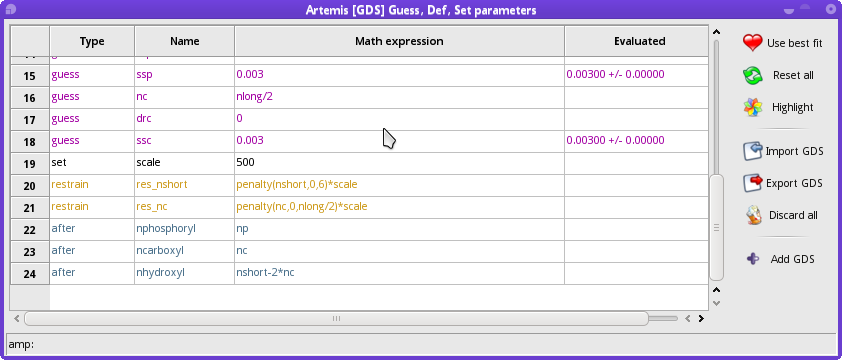
\includegraphics[width=\linewidth]{artemis/restraint.png}

    {\color{Orange3}Restraints} are managed on the Guess, Def, Set
    page, like any other parameter and will be properly used in the
    fit.  A restraint depends upon a {\color{Green4}def} or
    {\color{Magenta3}guess} parameters -- something that changes during
    the fit.
  \end{center}
\end{frame}

% \section[Artemis]{Bringing It All Together in Artemis}

% \againframe{themultiples}

% \begin{frame}
%   \frametitle{Artemis: Multiple $k$-Weights}
  
%   \begin{center}
%     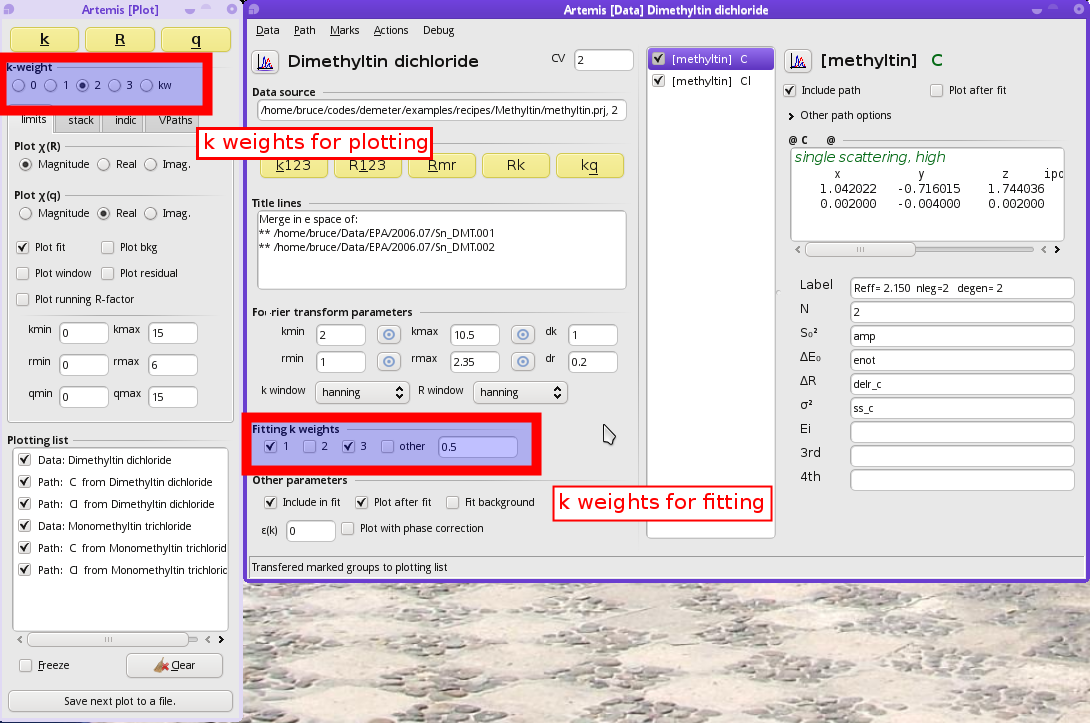
\includegraphics[width=0.9\linewidth]{artemis/mkw.png}

%     Simply click any/all of the fitting $k$-weight buttons.\\
%     Do not confuse them with the buttons that control k-weighting for
%     plots.
%   \end{center}
% \end{frame}

% \begin{frame}
%   \frametitle{Artemis: Multiple Feff Calculations}

%   \begin{center}
%     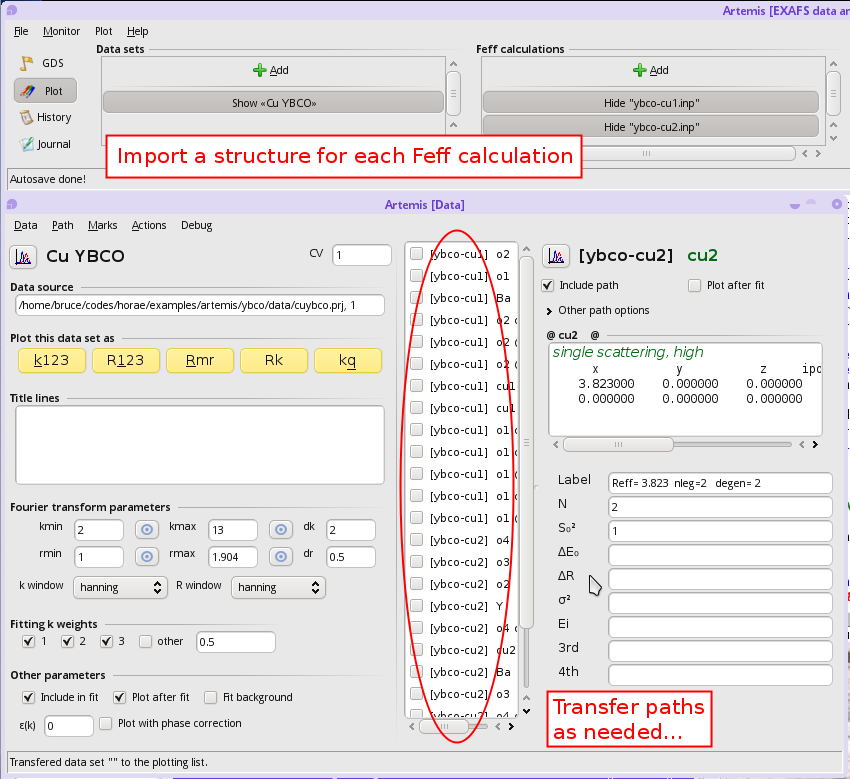
\includegraphics[width=0.6\linewidth]{artemis/mfc.png}

%     Use as many {\feff} calculations as you need, run {\feff}, import
%     and include whichever paths you need.  (\textit{Nota bene:} there
%     is an out-of-the-box limit of 128 paths in {\ifeffit}.)
%   \end{center}
% \end{frame}

% \begin{frame}
%   \frametitle{Artemis: Multiple Data Sets (I)}

%   If you have already imported data into {\artemis}, you can either
%   change the data on which you are working or import additional data
%   for a multiple data set fit,

%   \begin{center}
%     \includegraphics[width=0.2\linewidth]{artemis/change_data.png}\qquad
%     \includegraphics[width=0.4\linewidth]{artemis/data_import.png}
%   \end{center}

%   \begin{description}
%   \item[Change] From the ``Data'' menu in the Data window, select the
%     option to replace the $\chi(k)$.  This will open the file
%     selection dialog.
%   \item[New] Alternately, import data in the normal fashion.  It will
%     be added to the list of Data sets and included in all subsequent
%     fits.
%   \end{description}
% \end{frame}

% \begin{frame}
%   \frametitle{Artemis: Multiple Data Sets (II)}

%   \begin{center}
%     \includegraphics[width=0.6\linewidth]{artemis/mds.png}

%     Use as many data sets calculations as you need.  Each data set
%     needs one or more paths associated with it.  (\textit{Nota bene:}
%     there is an out-of-the-box limit of 10 data sets in {\ifeffit}.)
%   \end{center}
% \end{frame}

% \begin{frame}
%   \frametitle{Artemis: Specifying Constraints (I)}

%   In the uranyl example we saw earlier, the oxygen distances
%   associated with the mono- and bidentate ligands are at different
%   distances.
%   \begin{center}
%     \includegraphics[width=0.5\linewidth]{mfc/uranyl.png}    
%   \end{center}
%   The number of P atoms is equal to the number of shorter equatorial
%   oxygen atoms, while the number of C atoms is half the number of
%   longer equatorial oxygens.
% \end{frame}

% \begin{frame}
%   \frametitle{Artemis: Specifying Constraints (II)}

%   \begin{center}
%     \includegraphics[width=\linewidth]{artemis/constraint.png}

%     Constraints are implemented as {\color{Green4}def} parameter math
%     expressions.  (Path parameters can also be expressed as math
%     expressions.)  {\ifeffit}'s math expressions are quite expressive.
%   \end{center}
% \end{frame}

% \begin{frame}
%   \frametitle{Artemis: Specifying Restraints}

%   \begin{center}
%     \includegraphics[width=\linewidth]{artemis/restraint.png}

%     {\color{Orange3}Restraints} are managed on the Guess, Def, Set
%     page, like any other parameter and will be properly used in the
%     fit.  A restraint depends upon a {\color{Green4}def} or
%     {\color{Magenta3}guess} parameters -- something that changes during
%     the fit.
%   \end{center}
% \end{frame}

\section{Conclusion}

\begin{frame}
  \frametitle{Now you know all my tricks!}
  \LARGE
  \begin{block}{\LARGE Your assignment:}
    \begin{center}
      Use 'em all!

      \bigskip

      Do great data analysis!
    \end{center}
  \end{block}
\end{frame}

% \definecolor{MYcolor}{RGB}{163,137,47}   %% dirty yellow
% \section[Histograms]{Arbitrary Distribution Functions}
% \begin{frame}
%   \frametitle{Non-Gaussian Distributions}
% \end{frame}


\end{document}

%%% Local Variables:
%%% mode: latex
%%% TeX-master: t
%%% TeX-parse-self: t
%%% TeX-auto-save: t
%%% TeX-auto-untabify: t
%%% TeX-PDF-mode: t
%%% End:
